%%%%%%%%%%%%%%%%%%%%%%%%%%%%%%%%%%%%%%%%%
% Masters/Doctoral Thesis 
% LaTeX Template
% Version 1.43 (17/5/14)
%
% This template has been downloaded from:
% http://www.LaTeXTemplates.com
%
% Original authors:
% Steven Gunn 
% http://users.ecs.soton.ac.uk/srg/softwaretools/document/templates/
% and
% Sunil Patel
% http://www.sunilpatel.co.uk/thesis-template/
%
% License:
% CC BY-NC-SA 3.0 (http://creativecommons.org/licenses/by-nc-sa/3.0/)
%
% Note:
% Make sure to edit document variables in the Thesis.cls file
%
%%%%%%%%%%%%%%%%%%%%%%%%%%%%%%%%%%%%%%%%%

% Thesis should be printed on both sides of the paper. Use no less than 1.5 spacing, with quo- tations and notes single-spaced. Regarding Character size, not less than 2.0mm for capitals and 1.5mm for x-height (the height of a lower-case x). Us a serif font (i.e. Times) between 10 and 12 points. Use consistent and clear fonts through all the document.
% The text layout should be approximately as follows: • 4cm binding margin
% • 2cm head margin (top of page)
% • 2.5cm fore-edge margin
% • 4cm tail margin (bottom of page)

%  \parskip  \linespread{1.5}
%----------------------------------------------------------------------------------------
%	PACKAGES AND OTHER DOCUMENT CONFIGURATIONS
%----------------------------------------------------------------------------------------
% \documentclass[twoside,a4,12p]{report} 

%\documentclass[12pt, twoside]{Thesis} % The default font size and one-sided printing (no margin offsets)

\documentclass[twoside,a4,12p]{Thesis}

%\marginsize{4cm}{2.5cm}{4cm}{4cm}

%\usepackage{geometry}
%\marginsize{4cm}{2.5cm}{4cm}{4cm}

\graphicspath{{Pictures/}} % Specifies the directory where pictures are stored

\usepackage{subfigure}
\usepackage{float}
%\usepackage{graphics}
%\usepackage{graphicx}
\usepackage{bchart}
\usepackage{pgfplots}
%\usepackage{bm}
\usepackage[square, numbers, comma, sort&compress]{natbib} % Use the natbib reference package - read up on this to edit the reference style; if you want text (e.g. Smith et al., 2012) for the in-text references (instead of numbers), remove 'numbers' 
\hypersetup{urlcolor=blue, colorlinks=true} % Colors hyperlinks in blue - change to black if annoying
\title{\ttitle} % Defines the thesis title - don't touch this

\begin{document}

\frontmatter % Use roman page numbering style (i, ii, iii, iv...) for the pre-content pages

\setstretch{1.3} % Line spacing of 1.3

% Define the page headers using the FancyHdr package and set up for one-sided printing
\fancyhead{} % Clears all page headers and footers
\rhead{\thepage} % Sets the right side header to show the page number
\lhead{} % Clears the left side page header

\pagestyle{fancy} % Finally, use the "fancy" page style to implement the FancyHdr headers

\newcommand{\HRule}{\rule{\linewidth}{0.5mm}} % New command to make the lines in the title page

% PDF meta-data
\hypersetup{pdftitle={\ttitle}}
\hypersetup{pdfsubject=\subjectname}
\hypersetup{pdfauthor=\authornames}
\hypersetup{pdfkeywords=\keywordnames}

%----------------------------------------------------------------------------------------
%	TITLE PAGE
%----------------------------------------------------------------------------------------

\begin{titlepage}
\begin{center}

\textsc{\LARGE \univname}\\[1.5cm] % University name
\textsc{\Large Master Thesis}\\[0.5cm] % Thesis type

\HRule \\[0.4cm] % Horizontal line
{\huge \bfseries \ttitle}\\[0.4cm] % Thesis title
\HRule \\[1.5cm] % Horizontal line
 
\begin{minipage}{0.4\textwidth}
\begin{flushleft} \large
\emph{Author:}\\
\href{http://emreozanalkan.github.io}{\authornames} % Author name - remove the \href bracket to remove the link
\end{flushleft}
\end{minipage}
\begin{minipage}{0.4\textwidth}
\begin{flushright} \large
\emph{Supervisors:} \\
\href{http://camma.u-strasbg.fr}{\supname} % Supervisor name - remove the \href bracket to remove the link  
\end{flushright}
\end{minipage}\\[2cm]
 
\large \textit{A thesis submitted in fulfilment of the requirements\\ for the degree of \degreename}\\[0.3cm] % University requirement text
\textit{in the}\\[0.4cm]
% \groupname\\\deptname\\[2cm] % Research group name and department name
\deptname \\[0.4cm] % Research group name and department name
\textit{and carried at}\\[0.4cm]
Research Group CAMMA, ICube, University of Strasbourg\\[0.7cm]
 
{\large \today}\\[0.7cm] % Date
%\includegraphics{Logo} % University/department logo - uncomment to place it

\includegraphics[scale=0.4]{Figures/universiteBourgogneLogo} % University/department logo - uncomment to place it
% 
\includegraphics[scale=0.4]{Figures/strasbourgUniversityLogo}
% 
\includegraphics[scale=0.1]{Figures/hospitalLogo}
% 
\includegraphics[scale=0.15]{Figures/icubeLogo}
% 
\includegraphics[scale=0.4]{Figures/cammaLogoTransparent}
% 
\includegraphics[scale=0.5]{Figures/ihuLogo}
\vfill
\end{center}

\end{titlepage}

%----------------------------------------------------------------------------------------
%	DECLARATION PAGE
%	Your institution may give you a different text to place here
%----------------------------------------------------------------------------------------

\Declaration{

\addtocontents{toc}{\vspace{1em}} % Add a gap in the Contents, for aesthetics

I, \authornames, declare that this thesis titled, `\ttitle' and the work presented in it are my own. I confirm that:

\begin{itemize} 
\item[\tiny{$\blacksquare$}] This work was done wholly or mainly while in candidature for a master degree at this University.
\item[\tiny{$\blacksquare$}] Where any part of this thesis has previously been submitted for a degree or any other qualification at this University or any other institution, this has been clearly stated.
\item[\tiny{$\blacksquare$}] Where I have consulted the published work of others, this is always clearly attributed.
\item[\tiny{$\blacksquare$}] Where I have quoted from the work of others, the source is always given. With the exception of such quotations, this thesis is entirely my own work.
\item[\tiny{$\blacksquare$}] I have acknowledged all main sources of help.
\item[\tiny{$\blacksquare$}] Where the thesis is based on work done by myself jointly with others, I have made clear exactly what was done by others and what I have contributed myself.\\
\end{itemize}
 
Signed:\\
\rule[1em]{25em}{0.5pt} % This prints a line for the signature
 
Date:\\
\rule[1em]{25em}{0.5pt} % This prints a line to write the date
}

\clearpage % Start a new page

%----------------------------------------------------------------------------------------
%	QUOTATION PAGE
%----------------------------------------------------------------------------------------

\pagestyle{empty} % No headers or footers for the following pages

\null\vfill % Add some space to move the quote down the page a bit

\textit{``When David Marr at MIT moved into computer vision, he generated a lot of excitement, but he hit up against the problem of knowledge representation; he had no good representations for knowledge in his vision systems."}

\begin{flushright}
Marvin Minsky
\end{flushright}

%\vfill\null
\vfill\vfill\vfill\vfill\vfill\vfill\null % Add some space at the bottom to position the quote just right

 \clearpage % Start a new page

%----------------------------------------------------------------------------------------
%	ABSTRACT PAGE
%----------------------------------------------------------------------------------------

\pagestyle{empty} % No headers or footers for the following pages

\addtotoc{Abstract} % Add the "Abstract" page entry to the Contents

\abstract{\addtocontents{toc}{\vspace{1em}} % Add a gap in the Contents, for aesthetics

%\begin{abstract}


Operating room management and surgical procedure evaluation are time consuming tasks for operating room managers and clinicians. The demanding workload can be reduced thanks to context-aware system that use signals and data from operating rooms to automate processes such as surgical skill analysis, transcription of medical produces and evaluation of quality of procedures. Activity recognition is one of the key factors to enable the context-aware systems in the operating rooms. In this work, we address the problem of activity recognition in an operating room using a multi-view RGBD camera system. We adopt the activity recognition pipeline based on bag-of-words approach by \cite{twinanda2015data} and extend it with a 4D spatio-temporal voting scheme.  In the recognition pipeline, a data-driven non-rigid layout is learnt to divide the 4D spatio-temporal space of the features into 4D patches in order to recover the information loss caused by the bag-of-words approach. Since each patch from the learnt layout carries meaningful and semantic information of the 4D spatio-temporal space for an activity, the proposed voting scheme collects votes from the patches to determine the activity. We tested the proposed method on a multi-view RGBD dataset \cite{twinanda2015data} using two classifiers, i.e., Support Vector Machines (SVM) and Random Forest (RF). We also compare the results of the proposed voting scheme approach to the non-voting approach \cite{twinanda2015data}. The experiments show that the proposed voting scheme shows promising results with 83.1\% accuracy.

%\end{abstract}

}

% Operating room is a very important place where resource management and evaluation are very critical. Operating room management and evaluation bring many critical responsibilities such as surgical skill analysis, transcription of medical produces and evaluation of quality of procedures which cause high workload to clinicians and operating room managers. The high workload on operating room staff can be reduced  thanks to context-aware systems that use signals and data from operating rooms to automate processes. Activity recognition is indeed one of the key factors to enable the context-aware systems in the operating rooms. In this work, we address the problem of activity recognition in an operating room using a multi-view RGBD camera system. We adopt the activity recognition pipeline based on bag-of-words approach by \cite{twinanda2015data} and extend it with a 4D spatio-temporal voting scheme.  In the recognition pipeline, a data-driven non-rigid layout is learnt to divide the 4D spatio-temporal space of the features into 4D patches in order to recover the information loss caused by the bag-of-words approach. Since each patch from the learnt layout carries meaningful and semantic information of the 4D spatio-temporal space for an activity, the proposed voting scheme collects votes from the patches to determine the activity. We tested the proposed method on a multi-view RGBD dataset \cite{twinanda2015data} using various classifiers, i.e., Support Vector Machines (SVM) and Random Forest (RF). We also compare results of the proposed voting scheme approach to the non-voting approach \cite{twinanda2015data}. The experiments shows that the proposed voting scheme shows promising results with 83.1\% accuracy.


\clearpage % Start a new page

%----------------------------------------------------------------------------------------
%	ACKNOWLEDGEMENTS
%----------------------------------------------------------------------------------------

%\setstretch{1.3} % Reset the line-spacing to 1.3 for body text (if it has changed)

\acknowledgements{\addtocontents{toc}{\vspace{1em}} % Add a gap in the Contents, for aesthetics

I would first like to thank my supervisors Dr. Nicolas Padoy and Andru Putra Twinanda for all the support, valuable guidance and encouragement during this thesis. I would also like to thank my family for all their support\ldots

% I would first like to thank Dr. W. Samuel Easterling for his advice and guidance
% throughout the duration of this research. I would like to express sincere appreciation to
% Dr. Thomas M. Murray for his earnest efforts inside and outside of the classroom on my
% behalf and for serving on my committee. I would also like to thank Dr. Thomas E.
% Cousins for serving on my committee. Thanks also go to Nucor Corporation for
% sponsoring this research and to David Samuelson for his assistance throughout this
% project.
% I would like to express tremendous gratitude to my parents, Eric and Pauline
% Alander, for their constant love and support throughout my entire life and for providing
% me with the opportunity to further my education at the institute of my choice. A special
% thank you also goes to my fiancée, Gigi Kaldahl, for her encouragement, support, and
% understanding during my graduate studies.
% Many thanks go to Brett Farmer and Dennis Huffman for their hard work and
% invaluable help at the structures lab over the past year. Thanks also to Ann Crate for her
% assistance in preparing the data report for this study. A sincere thanks goes to Michelle
% Rambo-Roddenberry, Budi Widjaja, and Joe Howard for their assistance at the lab and
% from whom I have learned so much. I wish to express exceptional gratitude to Bobby
% Prince and Jared Jamison for their selfless help in the classroom and at the lab in the
% preparation of the test specimens for this project. Thanks also go to my fellow graduate
% students who were so helpful along the way. A special thanks is due Jennifer Frank, as
% well, for her assistance in the statistical analysis of the data presented in this report.
}

\clearpage % Start a new page

%----------------------------------------------------------------------------------------
%	LIST OF CONTENTS/FIGURES/TABLES PAGES
%----------------------------------------------------------------------------------------

\pagestyle{fancy} % The page style headers have been "empty" all this time, now use the "fancy" headers as defined before to bring them back

\lhead{\emph{Contents}} % Set the left side page header to "Contents"
\tableofcontents % Write out the Table of Contents

\lhead{\emph{List of Figures}} % Set the left side page header to "List of Figures"
\listoffigures % Write out the List of Figures

\lhead{\emph{List of Tables}} % Set the left side page header to "List of Tables"
\listoftables % Write out the List of Tables

%----------------------------------------------------------------------------------------
%	ABBREVIATIONS
%----------------------------------------------------------------------------------------

% \clearpage % Start a new page

% \setstretch{1.5} % Set the line spacing to 1.5, this makes the following tables easier to read

% \lhead{\emph{Abbreviations}} % Set the left side page header to "Abbreviations"
% \listofsymbols{ll} % Include a list of Abbreviations (a table of two columns)
% {
% \textbf{LAH} & \textbf{L}ist \textbf{A}bbreviations \textbf{H}ere \\
% %\textbf{Acronym} & \textbf{W}hat (it) \textbf{S}tands \textbf{F}or \\
% }

%----------------------------------------------------------------------------------------
%	PHYSICAL CONSTANTS/OTHER DEFINITIONS
%----------------------------------------------------------------------------------------

% \clearpage % Start a new page

% \lhead{\emph{Physical Constants}} % Set the left side page header to "Physical Constants"

% \listofconstants{lrcl} % Include a list of Physical Constants (a four column table)
% {
% Speed of Light & $c$ & $=$ & $2.997\ 924\ 58\times10^{8}\ \mbox{ms}^{-\mbox{s}}$ (exact)\\
% % Constant Name & Symbol & = & Constant Value (with units) \\
% }

%----------------------------------------------------------------------------------------
%	SYMBOLS
%----------------------------------------------------------------------------------------

% \clearpage % Start a new page

% \lhead{\emph{Symbols}} % Set the left side page header to "Symbols"

% \listofnomenclature{lll} % Include a list of Symbols (a three column table)
% {
% $a$ & distance & m \\
% $P$ & power & W (Js$^{-1}$) \\
% % Symbol & Name & Unit \\

% & & \\ % Gap to separate the Roman symbols from the Greek

% $\omega$ & angular frequency & rads$^{-1}$ \\
% % Symbol & Name & Unit \\
% }

%----------------------------------------------------------------------------------------
%	DEDICATION
%----------------------------------------------------------------------------------------

\setstretch{1.3} % Return the line spacing back to 1.3

\pagestyle{empty} % Page style needs to be empty for this page

\dedicatory{Dedicated to my professors\ldots} % Dedication text

\addtocontents{toc}{\vspace{2em}} % Add a gap in the Contents, for aesthetics

%----------------------------------------------------------------------------------------
%	THESIS CONTENT - CHAPTERS
%----------------------------------------------------------------------------------------

\mainmatter % Begin numeric (1,2,3...) page numbering

\pagestyle{fancy} % Return the page headers back to the "fancy" style

% Include the chapters of the thesis as separate files from the Chapters folder
% Uncomment the lines as you write the chapters

% Chapter 1

\chapter{Introduction} % Main chapter title

\label{Chapter1} % For referencing the chapter elsewhere, use \ref{Chapter1} 

\lhead{Chapter 1. \emph{Introduction}} % This is for the header on each page - perhaps a shortened title

%----------------------------------------------------------------------------------------

Activity recognition using cameras is a very active research topic since the past several decades in the domain of computer vision. It has been widely applied in many fields, such as video surveillance, human computer interaction, robotics and medicine. However, activity recognition is still a very challenging problem due to the large amount of data, amount of computational power required, and high intra-class variations of activities. Over the past decades, researchers have mainly focused on using image sequences from single-view RGB cameras for activity recognition which have many inherent limitations. Single-view camera approaches have limitations due to narrow field of view which makes it more vulnerable to occlusions. Moreover, RGB cameras are very sensitive to illumination changes. 

Thanks to recent technological advances and the emergence of cost-effective depth sensors, depth cameras have become more popular and attracted many researchers to use them in activity recognition studies. Depth sensors have many advantages over RGB cameras. For example, they can provide structural information of the scenes and they can even work in total darkness since infrared structured light is used to reconstruct the scenes. All these advantages make it interesting to incorporate the RGBD cameras into a more challenging environments, e.g., operating rooms (OR).

Recent progresses in medicine transformed operating rooms into hybrid rooms equipped with new imaging devices, robotic arms, sensors and electronic devices. These changes require more management and tracking of information. Therefore, activity recognition in operating rooms has become an important research field in the domain of medicine. It enables applications, such as OR time management for hospitals \cite{Bhatia:2007:RIO:1620113.1620126}, surgical work-flow modeling and monitoring \cite{DBLP:journals/tbe/LalysRBJ12, Padoy2012632}, surgical skill analysis \cite{Zappella2013732} and automatic transcription of medical procedures \cite{6553758}. In particular, activity recognition in operating rooms equipped with x-ray imaging devices can be used to estimate  the radiation exposure of the patients and the clinicians and correlate it to their activities \cite{seeingIsBelievingNL}. 

In order to recognize activities, many data sources from operating rooms can be used, e.g, the vital signs of the patients \cite{Bhatia:2007:RIO:1620113.1620126} and tool usage signals \cite{Padoy2012632}. However, they are only providing local information that is not enough to capture global activities and events in the operating room. Thus, in this thesis, we focus on performing activity recognition on videos. Specifically we are identifying what activities is happening in a video clip.

\citet{twinanda2015data} have addressed the same problem. In their work, they proposed an action recognition pipeline with a novel feature encoding scheme that achieved 85.53\% accuracy. The proposed novel feature encoding extends the bag-of-words (BoW) approach to learn a data-driven non-rigid layout to divide the 4D spatio-temporal (3D spatial + 1D temporal) space of the feature locations. Their work showed that encoding features with the learned non-rigid layout retains more spatio-temporal information compared to the rigid counterpart, i.e, SPM \cite{1641019}. 

In this thesis, we propose to adopt the activity recognition pipeline from \cite{twinanda2015data} and extend it with a voting scheme to solve activity recognition in the operating room. Firstly, spatio-temporal interest points (STIP) and depth spatio-temporal interest points (DSTIP) are detected from intensity and depth video clips respectively. Secondly, histogram of optical flows (HOF) from intensity and depth cuboid similarity features (DCSF \cite{6619209}) from depth data are extracted around the detected interest points. Then we learn two separate dictionaries to encode our extracted features. A visual dictionary is learned to encode visual features: the HOF and the DCSF \cite{6619209}. On the other hand, the spatio-temporal dictionary is learned to define a 4D non-rigid layout. The non-rigid layout divides the 4D spatio-temporal space into smaller 4D patches. From each patch, a histogram of feature points will be counted. Finally, histograms coming from the same video clip will be passed to the classifiers to vote for the action. We also introduce two voting approaches: one-model and multi-model. In the one-model approach, each patch from all video clips are used to train a classifier. On the other hand, the multi-model approach trains a separate classifier for each patch. In order to provide a comprehensive comparison, we present the results for voting sheme and non-voting scheme approaches using non-linear SVM and Random Forest classifiers.

The rest of the thesis is organized as follows. Chapter~\ref{Chapter2} introduces the related work on activity recognition. Chapter~\ref{Chapter3} provides the details of the methodology used in this work. Chapter~\ref{Chapter4} describes and discusses the experimental setup and results. Finally, Chapter~\ref{Chapter5} presents the conclusions of the thesis. 




% Chapter 2

\chapter{Related Work} % Main chapter title

\label{Chapter2} % For referencing the chapter elsewhere, use \ref{Chapter2} 

\lhead{Chapter 2. \emph{Related Work}} % This is for the header on each page - perhaps a shortened title

%----------------------------------------------------------------------------------------
%	RELATED WORK
%----------------------------------------------------------------------------------------
% TODO: 
% 	+ BoW approach of related works should be added
%	+ Maybe SPM can be more given in more details

	The problem of activity recognition has been widely studied in the computer vision field. Recent works show excellent performances using local features such as local motions \cite{5995407, 6909503}, human detectors \cite{Klaser:2010:HFA:2435051.2435071} and skeleton tracking \cite{6909731, 6909476, 6909493}. In \cite{6909503}, Yang et al. presented an activity recognition framework for depth sequences. Clustered hypersurface normals are used to construct polynormals to get shape information from depth sequences. The method achieved good results on public Microsoft human action dataset MSR \cite{MSR:5543273, MSR:6618942, MSR:Wang:2012:RAR:2403006.2403071, MSR:6247813}. However, super normal vectors (SNV) encoded method is not reliable either on a highly cluttered and occluded environment or when the actions have very low depth variance.

	More recently, great improvements were obtained by using skeleton tracking based activity recognition approaches. \citet{6909476} proposed a novel skeleton representation that is modeling the 3D geometric relationships between various body parts. They outperformed most of the skeleton-based state-of-the-art methods with their representation. In other work, \citet{6909731} argues that skeleon-based approaches are limited by the effective working distance of the RGBD cameras and practically they are not online all the time. They proposed using the combination of intensity, depth and skeleton structures. In \cite{6909735}, Want et al. stated that action recognition is view-dependent and proposed a novel multiview spatio-temporal graphical representation for cross-view action recognition. The proposed method leverages from 3D human skeleton data. Despite the satisfactory performance of skeleton tracking approaches, frontal camera views of the persons with low occlusion is needed which are not always possible in environments such as the operating rooms. \citet{RahimKinectOR} addressed the problem of skeleton tracking of clinicians in the operating rooms and showed that off-the-shelf skeleton tracking methods fail most of the time.
    
 	In one of the most related work with a multi-view systems and voting scheme, \citet{Zhu201320} addressed the problem of multi-view activity recognition using voting scheme and random forest classifier. They use IXMAS human action dataset \cite{IXMAS:weinland06, IXMAS:weinland10a} which consist of 5 cameras, 13 daily-live actions with various data, e.g., silhouettes, reconstructed volumes. However, the dataset does not consist of real activities, i.e., the dataset is recorded in a laboratory environment. The method is dependent on the extracted 2D silhouettes from each camera. The segments in temporal domain consist of 2D binary silhouettes which are used to train the Random Forest classifier to get prediction histograms used in voting. The voting strategy collects the vote from each segment of video clip and apply the weights on the features and on the camera views. This voting strategy is different than our proposed voting scheme where we divide 4D space into cells to collect votes. Their results showed that combination of multi-view cameras, voting scheme and Random Forest classifier produce good results. On the other hand, in multi-view camera systems, actions may not be available from each camera view all the time. Furthermore, methods like silhouette extraction, human tracking are not feasible solutions to be used in high cluttered and occluded environment, e.g., the crowded places, operating rooms etc.
    
    Similarly, in this thesis, we address the problem of activity recognition in the operating room using a multi-view camera system. It is not a trivial problem because of various challenges. Firstly, camera positioning in operating rooms for better field of view while accommodating the articulation of the surgical equipments is very challenging. In addition, operating rooms are very dense and dynamic with a cluttered background and reflective objects, high occlusions, illumination changes , upfront camera view and very tiny or slow movements. Hence, methods in \cite{6909503, 6909476, 6909731,6909735, Zhu201320} are not sufficient to deal with these problems. Due to these difficulties, it is required to have lower level features to represent the video clips.
    
    One example of the lower level features for an image sequence is spatio-temporal interest point (STIP)\cite{ laptev2005space}. STIPs are sparse interest points along spatial and temporal domain, which are detected by Harris corner detection in 3D spatio-temporal domain. In \cite{1570899}, Dollar et al. proposed a modified sparse and informative STIP and showed that it is robust to pose, clutters and occlusions. The STIPs \cite{1570899} are described with cuboids extracted from surrounding spatio-temporally windowed data. The proposed interest points are more robust to gradual gradient changes and periodic movements. However, the approach was designed to work mainly for intensity data and did work properly on depth data because of the nouse. \citet{6619209} proposed filtering method to detect STIP in depth data, namely depth spatio-temporal interest points (DSTIP). They also introduced a novel feature (i.e., Depth Cuboid Similarity Feature) to describe local similarity of 3D depth cuboids around DSTIP.
    
    In a recent work, \citet{twinanda2015data} showed that intensity or depth data is not sufficient by itself to recognizing some actions in the operating rooms. Some actions are well recognized in depth videos due to illumination problems in intensity data, and some actions give better results in intensity data due to low depth variance of depth data. Hence, the combination of both intensity and depth data have more discriminating power than using only intensity or depth data. The problem of activity recognition in an operating room using multi-view RGBD camera systems was addressed. A dataset of 1734 video clips of 15 surgical activity is generated using 2 RGBD cameras from real surgical operations in a hybrid operating room. Then, STIP \cite{1570899} and DSTIP \cite{6619209} are detected from intensity and depth respectively. They extracted Histogram of Optical Flows (HOF) and Depth Cuboid Similarity Feature (DCSF \cite{6619209}) features around the STIP and DSTIP respectively. These features are encoded by a novel feature encoding scheme that extends the bag-of-words (BoW) approach to learn a non-rigid layout that divides the 4D spatio-temporal space of the feature locations. Achieving 85.53\% accuracy, the work showed that encoding features with the non-rigid layout retains more spatio-temporal information compared to Spatial Pyramid Matching (SPM) \cite{1641019}.


 
% Chapter 3

\chapter{Methodology} % Main chapter title

\label{Chapter3} % For referencing the chapter elsewhere, use \ref{Chapter3} 

\lhead{Chapter 3. \emph{Methodology}} % This is for the header on each page - perhaps a shortened title

%----------------------------------------------------------------------------------------

	In this section, the adopted activity recognition pipeline from \cite{twinanda2015data} and the proposed voting scheme are explained in detail with various classification strategies.

%----------------------------------------------------------------------------------------

\section{Adopted Classification Pipeline \citep{twinanda2015data}}
\label{section:AdoptedClassificationPipeline}
The adopted pipeline \cite{twinanda2015data} is as follows: acquisition from a multi-view camera setup, interest point detection, feature extraction and building a data-driven non-rigid layout for feature encoding.

%----------------------------------------------------------------------------------------
\subsection{Multi-View RGBD Camera Setup}
\label{section:MultiViewRGBDCameraSetup}
    The proposed multi-view camera system contains two RGBD sensors, i.e. Asus XtionPro Live, mounted on the ceiling of the operating room. The cameras record both intensity and depth data synchronously at 14 fps with 640 x 480 resolution. While one of the sensors is capturing the area around the operating room bed, the other sensor captures the area with equipment table, in which large area of the operating rooms is covered.
    Furthermore, thanks to minimal overlapping of the views of the sensors, interference of infrared patterns of depth sensors are very less. The intrinsic parameters for each camera are obtained by calibration with checkerboard pattern. The extrinsic parameters are obtained  by using laser pointer method described in \cite{7035826}. Both camera views are shown in \ref{fig:cameraViews}. Panoramic view of the operating room that is showing the camera setups is provided in Appendix~\ref{AppendixA}.
    
\begin{figure}
\centering
\subfigure[Camera view 1 - intensity data]{\label{sfig:view1Intensity}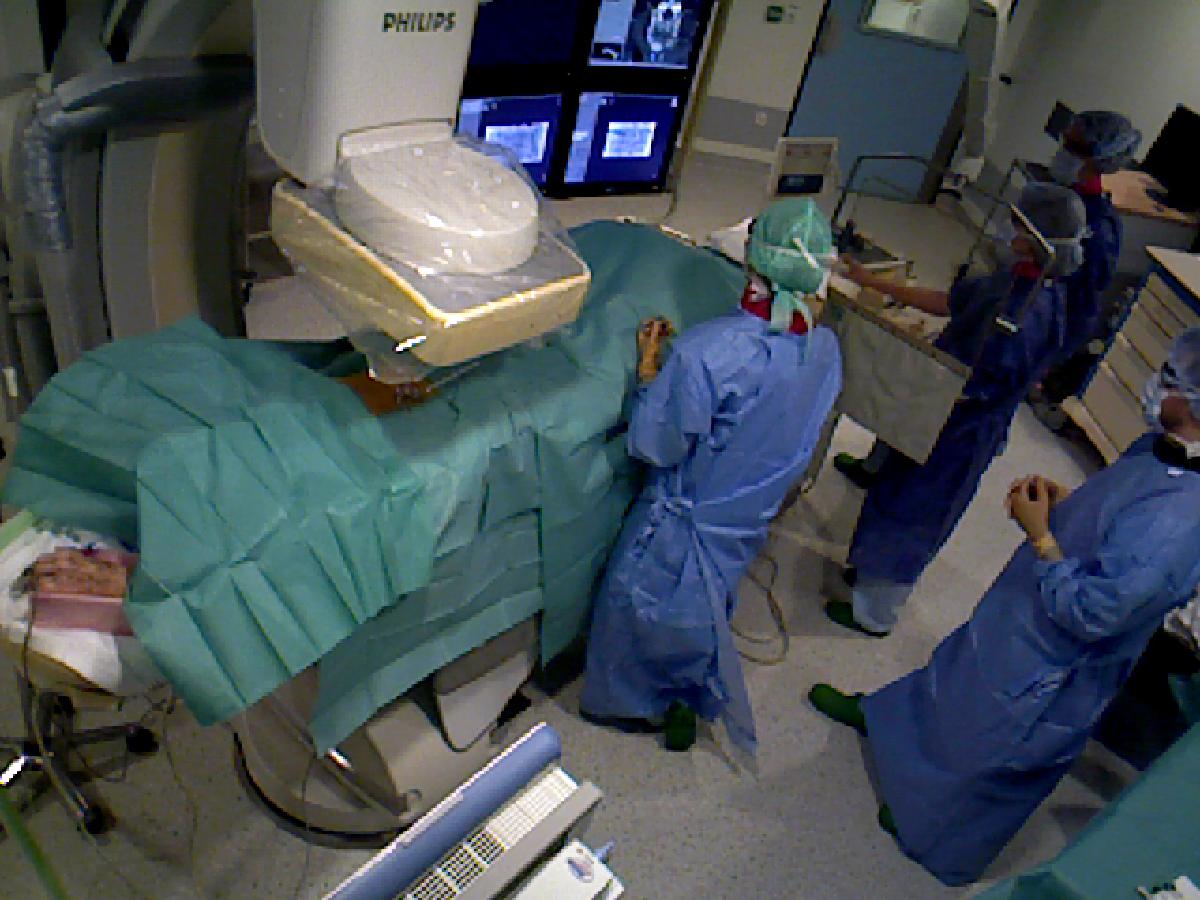
\includegraphics[width=.5\textwidth]{Figures/View1Color}}\hfill
\subfigure[Camera view 1 - depth data] {\label{sfig:view1Depth}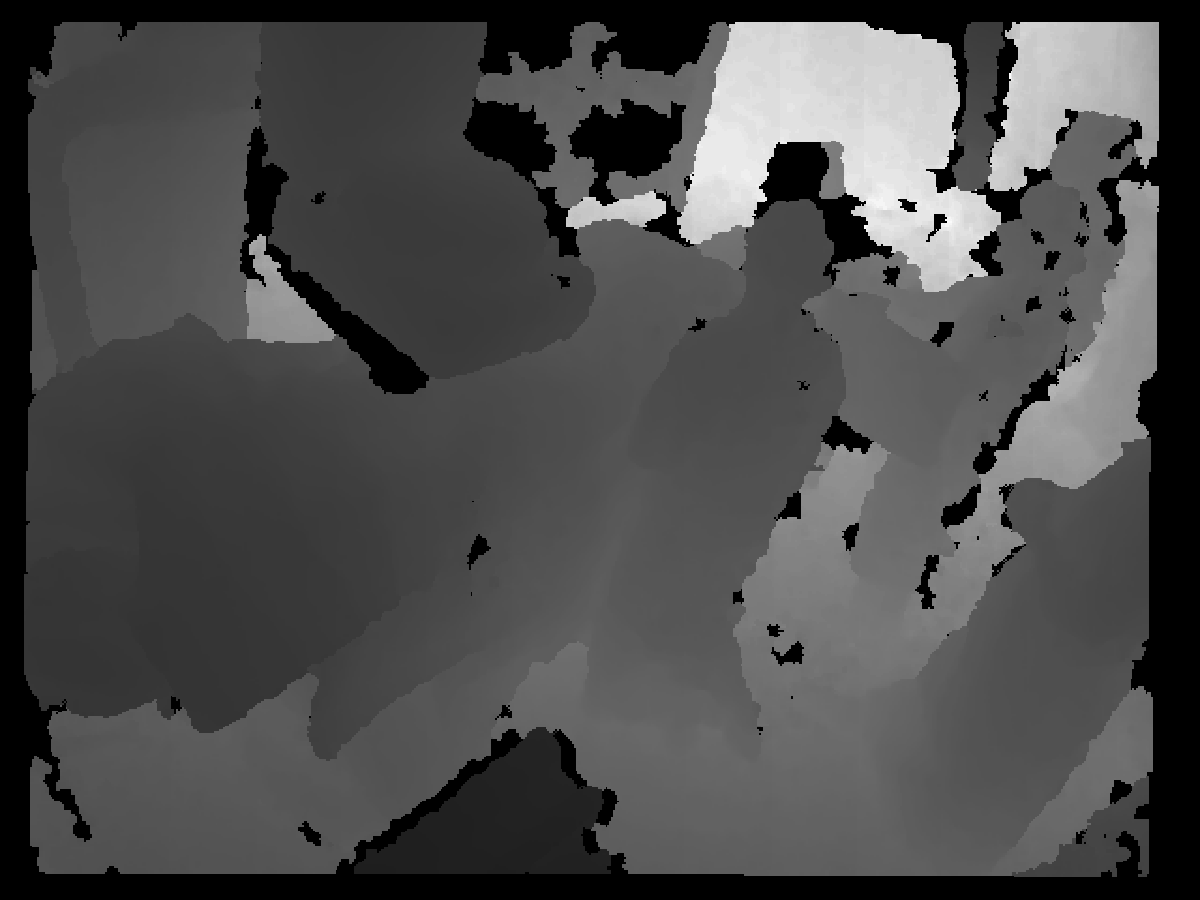
\includegraphics[width=.5\textwidth]{Figures/View1Depth}}\\
\subfigure[Camera view 2 - intensity data]{\label{sfig:view1Intesity}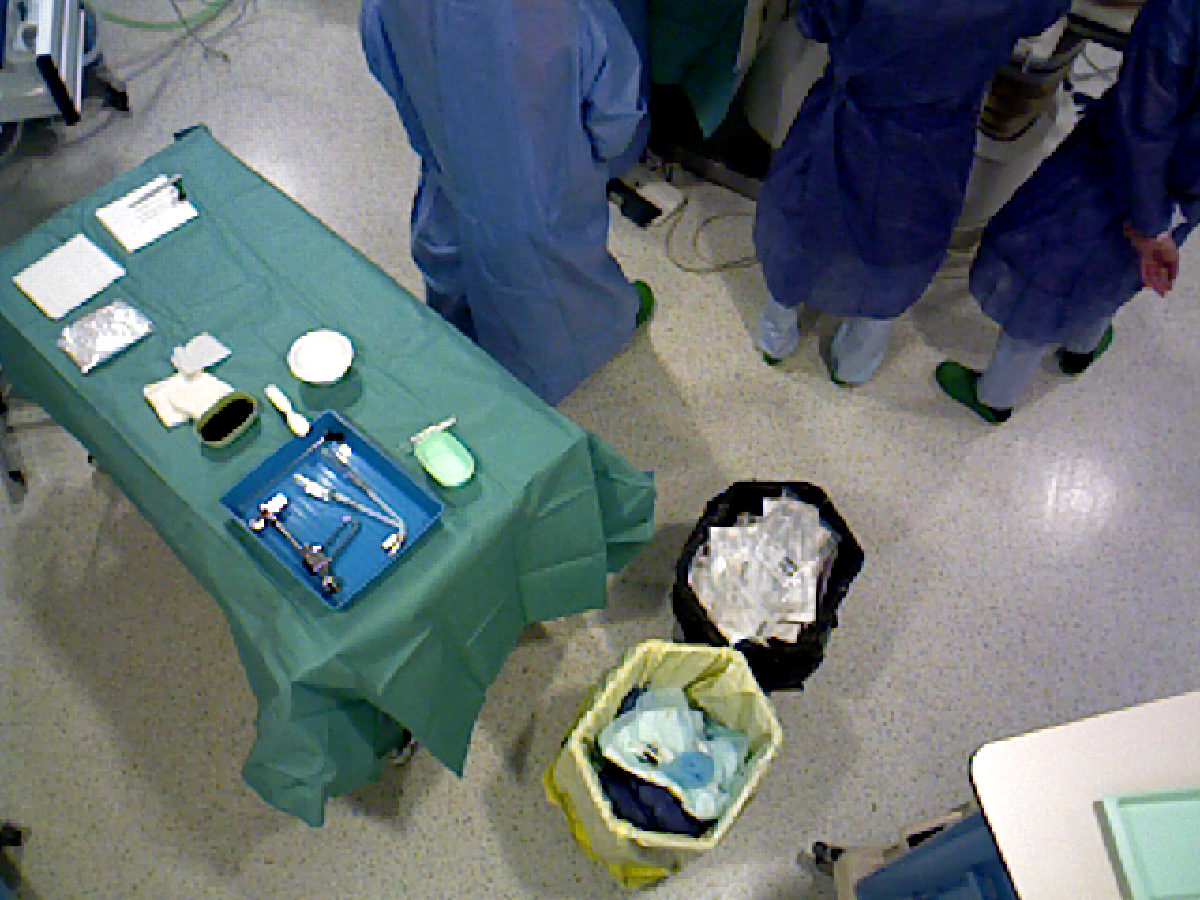
\includegraphics[width=.5\textwidth]{Figures/View2Color}}\hfill
\subfigure[Camera view 2 - depth data]{\label{sfig:view2Depth}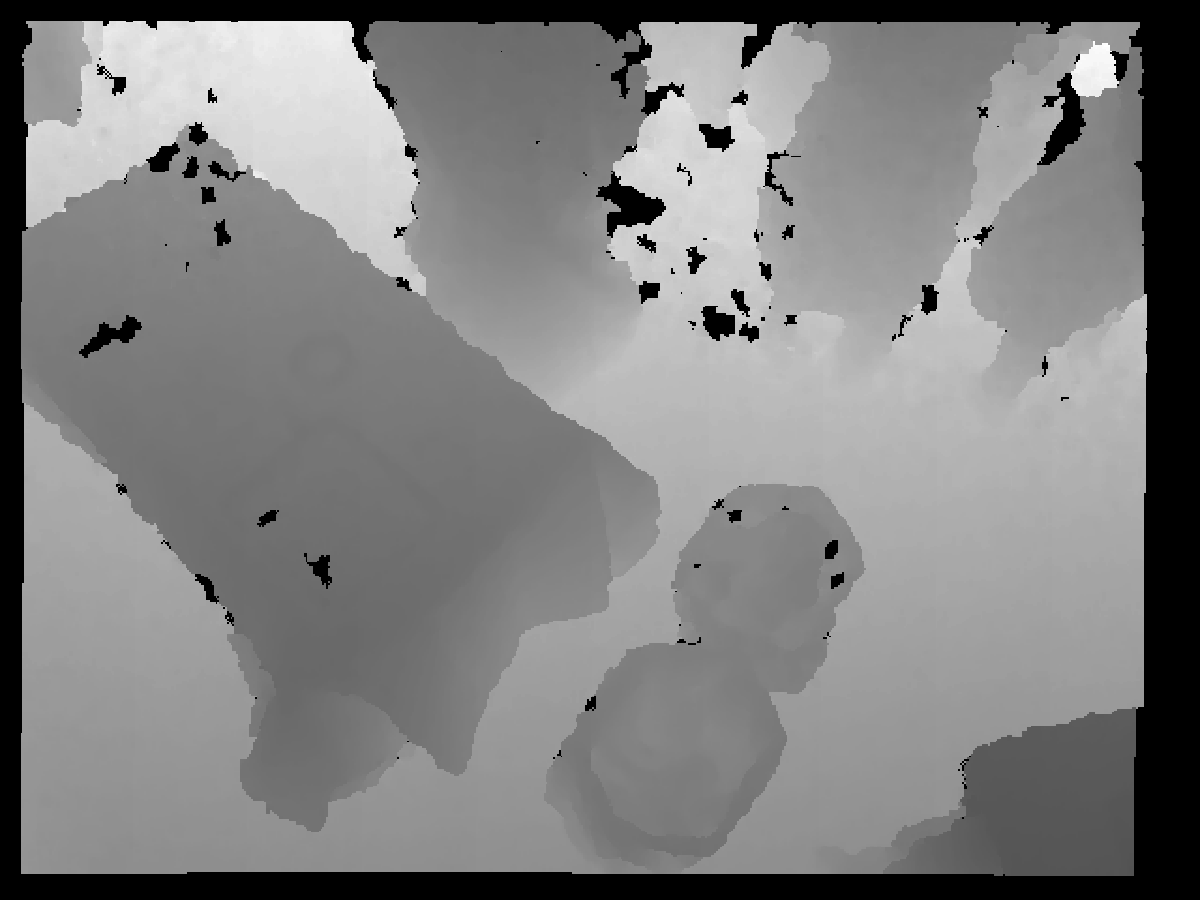
\includegraphics[width=.5\textwidth]{Figures/View2Depth}}\\
\caption{Sample images from RGBD sensors with view 1 and view 2.}
\label{fig:cameraViews}
\end{figure}
%----------------------------------------------------------------------------------------
\subsection{Interest Point Detection}
\label{section:InterestPointDetection}
	In the activity recognition pipeline, spatio-temporal interest points (STIP) by \citet{1570899} are used for intensity data. STIPs are computed by applying separable linear filters to get local maximum of the response. The response fuction $R$ of an intensity image $I$ is calculated as follows:

\begin{equation}
R_{I} = \left(I * g * h_{even}\right)^{2} + \left(I * g * h_{odd}\right)^{2},
\label{eq:stipResponseFunction}
%\nonumber
\end{equation}

	where $g(x, y; \sigma)$ is the 2D Gaussian smoothing kernel with scale $\sigma$, applied on the spatial $\left(x, y\right)$ dimensions. Terms $h_{even}$ and $h_{odd}$ are the quadrature pair of 1D Gabor filters applied in temporal domain defined as: $h_{even}\left(t|\tau,\omega,\right)=\cos\left(2\pi\omega t\right)e^{\frac{-t^{2}}{2\tau^{2}}}$ and $h_{odd}\left(t|\tau,\omega\right)=\sin\left(2\pi\omega t\right)e^{\frac{-t^{2}}{2\tau^{2}}}$.
    
    However, the STIP detector does not perform well and falsely detected on depth data because of the nature of the depth data where it may contain noise from sensors, pattern interference and fast foreground/background change of the border pixels. In order to cope with these problems, DSTIP detector by \citet{6619209} is used to detect depth spatio-temporal interest points (DSTIP) on depth data which introduced filtering method to reduce the noise and the false detection. Additional noise suppression term is proposed for noise filtering to equation \ref{eq:stipResponseFunction}:

\begin{equation}
R_{D} = \left(D * g * h_{even}\circ\bar{s}\right)^{2}+\left(D * g * h_{odd}\circ\bar{s}\right)^{2},
\label{eq:dstipResponseFunction}
%\nonumber
\end{equation}

where $D$ is the depth image, and $\bar{s}$ is the noise suppression term.


%----------------------------------------------------------------------------------------
\subsection{Feature Extraction}
\label{section:FeatureExtraction}
We compute features by extracting 3D cuboid around each detected interest points in spatio-temporal location $\left(x, y, t\right)$. Thus, the cuboids are the spatio-temporally windowed pixel values that contain most of the data contributed to response function \ref{eq:stipResponseFunction} and \ref{eq:dstipResponseFunction} to detect interest points. The size of the cuboids $\left(\Box_{x}\times\Box_{y}\times\Box_{t}\right)$ is proportionally assigned according to the spatial scale $\sigma$ and the temporal scale $\tau$.

Intensity cuboids are extracted from intensity data and histograms of optical flow (HOF) are calculated from the intensity cuboids. HOFs are used in intensity feature extraction process due to its distinguishable properties for direction of motion. These properties help to distinguish activities which have similar movements with different directions.

Moreover, 3D depth cuboids are extracted from depth data. Then, the depth cuboid similarity features (DCSF) \cite{6619209} are computed from the cuboids. DCSFs are computed based on self-similarity to encode spatio-temporal structure of the 3D cuboid. DCSF divides cuboids into smaller voxels, compute histograms of the depth pixels from each voxel, calculating relationship of each voxel by defining similarity between voxels using Bhattacharyya distance, then combination of all similarity scores from the voxels are concatenated to generate a DCSF feature.

%----------------------------------------------------------------------------------------
\subsection{Data Driven Feature Encoding}
\label{section:DataDrivenFeatureEncoding}

	The bag-of-words (BoW) is a model that treats image features as words to construct vocabulary. Then, histogram of occurrences of the words from the vocabulary produces a sparse histogram vector. $K$-means is typically used to encode the features which provide a global representation with BoW where $\mathbf{x}$ is a feature, $ \forall \mathbf{x} $, a value $w\in\left\{ 1,\cdots,K\right\}$, where $K$ is number of $K$-means center, is assigned to describe the index of the $K$-mean center which is the closest to feature $\mathbf{x}$. Hence $K$-means clusters every feature vector $\mathbf{x}\in\mathbb{R}^{n}$ and express them in a sparse representation $\mathbf{s}\in\mathbb{R}^{K}$ which is the occurrences of the words from the learnt dictionary $\mathbf{D}\in\mathbb{R}^{n\times K}$

	In \cite{twinanda2015data}, learning two separate dictionaries are proposed: a visual dictionary $\mathbf{D_{v}}$ with $K_{v}$ centers and a spatio-temporal dictionary $\mathbf{D_{st}}$ with $K_{st}$ centers. The visual dictionary $\mathbf{D_{v}}$ is learnt for encoding the visual features, i.e., the HOF and the DCSF for representing video clips. On the other hand, the spatio-temporal dictionary $\mathbf{D_{st}}$ is learnt by clustering the locations of the interest points $\left(x,y,z,t\right)$, where $X=\left(x,y,z\right)$
and $t$ are the 3D coordinates and the temporal location
of the interest point, respectively. Since the video clips varies in length, $t$ is normalized by length of its video clip. Multi-view camera systems require to define one camera's coordinate system as a reference coordinate system to transform the 3D coordinates into a common coordinate system. Hence, the final 3D coordinates are computed by:

\begin{equation}
\begin{array}{c}
X=T_{R}\cdot Y+T_{t}\\
Y=d\cdot C^{-1}\cdot\left(\begin{array}{ccc}
u & v & 1\end{array}\right)^{\top},
\end{array}
\end{equation}

where $Y$ is the 3D point in the camera frame, $\left(u,v\right)$
and $d$ are respectively the image pixel coordinates and the corresponding
depth value, $C$ is the intrinsic camera matrix, $T_{R}$
and $T_{t}$ are respectively the rotation and translation from the
camera frame to the reference frame. Then, learnt spatio-temporal dictionary $\mathbf{D_{st}}$ is used to place a non-rigid spatio-temporal grid to divide the spatio-temporal space into patches $\{P^{1},...,P^{K_{st}}\}$. These local patches from the non-rigid layout are high dimensional 4D patches. One example of feature encoding in 2D space is shown in Figure~\ref{fig:featureEncoding} where non-rigid layout is learnt by clustering points indicated with colored patches and features are extracted from the patches.

\begin{figure}[htbp]
\begin{center}
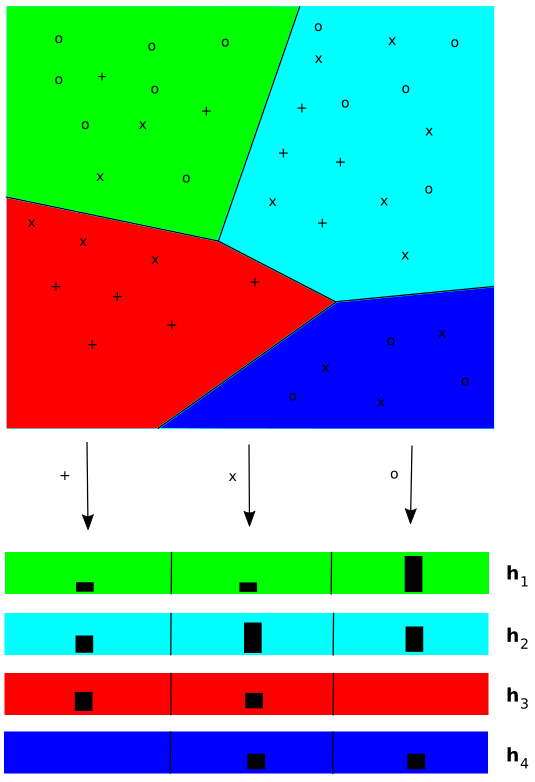
\includegraphics[scale=0.5]{Figures/featureEncoding}
\end{center}
\caption{Example of data driven feature encoding in 2D space with $K_{v}$ = 3 and $K_{st}$ = 4\label{fig:featureEncoding}}
\end{figure}
    
	In order to get the final histogram representation of the patches for a video clip $V_{i}$, where $i$ is video instance count, firstly, all features, $\forall \mathbf{x}$, belong to their corresponding patch, $P^{j}$, are found using the $\mathbf{D_{st}}$. Secondly, using the $\forall \mathbf{x} \in P^{j}$, the histogram of visual word occurrences from every patch $P^{j}$ is computed using $\mathbf{D_{v}}$. Finally, we obtain $K_{st}$ histograms, $\{_{i}H^{1},..., _{i}H^{K_{st}}\}$, representing the patches $P^{j}$ from video clip $V_{i}$, where $_{i}H^{j} \in \mathbb{R}^{K_{v}}$.
%----------------------------------------------------------------------------------------
\section{Voting Scheme}
\label{section:VotingScheme}
We extended the pipeline aforementioned by proposing a voting scheme. The proposed voting scheme uses histograms $H^{j}$ obtained from patches $P^{j}$ of a data-driven non-rigid layout presented in Section~\ref{section:DataDrivenFeatureEncoding}. We classify every local patch $P^{j}$ using $H^{j}$ independently and collect their vote for calculating majority vote for global activity. Hence every patch $P^{j}$ holds information about activity with semantic information that is contributing globally. 

%----------------------------------------------------------------------------------------
\section{Activity Classification}
\label{section:ActionClassification}

	In our multi-view camera system, every activity $a_{i}$ is recorded from both of the views. Hence, it produces a video clip pair $\left(V_{i}^{1},V_{i}^{2}\right)$ from the cameras. Firstly, interest point detection in Section~\ref{section:InterestPointDetection} is applied on the video clip pair $\left(V_{i}^{1},V_{i}^{2}\right)$ and features are extracted as described in Section~\ref{section:FeatureExtraction}. Then, two dictionaries are learnt for encoding as described in Section~\ref{section:DataDrivenFeatureEncoding}. The learnt spatio-temporal dictionary divides 4D space into smaller local 4D patches $\{P^{1},...,P^{K_{st}}\}$. Then, histogram representation $H^{j}$ from each local patch $P^{j}$ is calculated using the learnt visual dictionary for the video clip pair $\left(V_{i}^{1}, V_{i}^{2}\right)$. In order to get final histogram representation, $\{_{i}H^{1},..., _{i}H^{K_{st}}\}$, for video clip pair $\left(V_{i}^{1},V_{i}^{2}\right)$, we merge information by computing $_{i}H^{j} = _{i}^{1}H^{j} + _{i}^{2}H^{j}$ where $_{i}^{1}H^{j}$ and $_{i}^{2}H^{j}$ are respectively histograms from patch $P^{j}$ of $V_{i}^{1}$ and $V_{i}^{2}$. Then, final histograms, $\{H^{1},..., H^{K_{st}}\}$ from all video clip pairs are passed to the classifier for training and testing. In order to make performance comparison, we use the one-against all Support Vector Machine (SVM) with the nonlinear kernel, and we use Random Forest implementation to give comprehensive comparison of the voting scheme.

\subsection{SVM}
\label{section:SVM}
Support Vector Machine (SVM) is a well known supervised machine learning model for classification and regression. It uses hyper-planes in high dimensional space to divide training data with largest margin of the points. In this work, non-linear SVM with Chi-square $ \left(\mathcal{X}\right)^{2} $ and histogram intersection kernel is used. Since we have multi-class problem, we use one-against-all SVM to handle multi-class problem.



\subsection{Random Forest}
\label{section:RandomForest}
Random Forest is an algorithm of ensemble learning methods that used for classification and other tasks. Random Forest is collection of multiple decision trees that each produces a probabilistic response of the prediction of the classes with bagging and random selection of features. Then, these responses are combined to construct prediction which reduces over-fitting problem of the single decision tree models. Random Forest can be thought as a group of weak learners combined to get stronger learner.



\subsection{Training Strategy}
\label{section:TrainingStrategy}
In this work, we propose to use a two-level classification strategy to carry on the voting scheme. In the first level, we learn a classification model to obtain the probability votes from the 4D patches. However, in the second level classification, we learn the weights for the probability votes under the assumption that each patch has different contribution. In addition to the proposed training strategy, we also propose to use two different approaches used in the first level of the proposed classification strategy, i.e., one-model and multi-model approaches. In the one-model approach, all histograms from each patch from each video is trained using one classifier. However, in the multi-model approach, separate classifiers are trained for each patch.

\subsubsection{One-Model Approach}
\label{section:OneModelApproach}
In one-model approach, we use one classifier model in each level, i.e., $M_{level1}$ and $M_{level2}$. First, we train $M_{level1}$ with the training set which consists of a collection of histogram vectors $\{H^{1}, ..., H^{K_{st}}\}$. Then, we pass the histogram vectors to $M_{level1}$ to get the probability votes $\{W^{1}, ..., W^{K_{st}}\}$ from each video clip pair where $W^{j} \in \mathbb{R}^{N_{c}}$ and $N_{c}$ is the number of activity classes. Then, we concatenate the probability vectors, $W = \left[(W^{1})^{T}, ..., (W^{K_{st}})^{T}\right]^{T}$ where $W \in \mathbb{R}^{N_{c} \cdot K_{st}}$, of the same video clip. Finally, we train the second level classifier model $M_{level2}$ with the concatenated probability vectors $W$. Testing is done with same order: (1) testing set is passed through the first level classifier model $M_{level1}$ and the probability votes from the same video clips are concatenated, (2) concatenated probability votes are passed through the second level model $M_{level2}$ to to get the final classification probability. An illustration of the one-model approach is shown in Figure~\ref{fig:oneModelApproachIllustration}.
    
\begin{figure}[!htbp]
\begin{center}
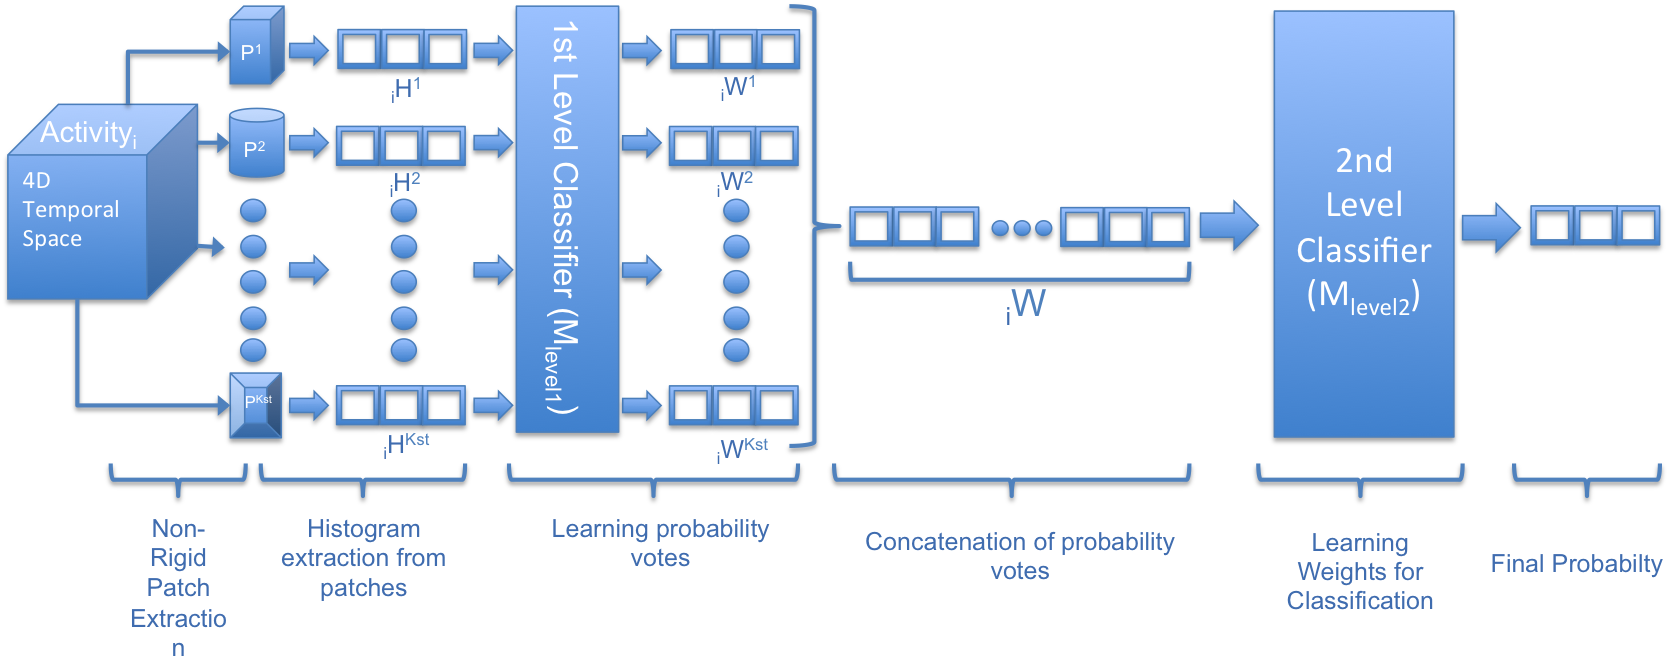
\includegraphics[scale=0.50]{Figures/oneModelApproach3}
\end{center}
\caption{Illustration of one-model approach to classify a video clip \label{fig:oneModelApproachIllustration}}
\end{figure}


\subsubsection{Multi-Model Approach}
\label{section:MultiModelApproach}
In contrast to the one-model approach, we propose to use multiple classifiers in the first level classification. Each patch $P^{j}$ in the first level classification has its own classifier model, i.e., $\{M_{level1}^{1},\dots,M_{level1}^{K_{st}}\}$. In order to train the first level classifiers, $\{M_{level1}^{1},\dots,M_{level1}^{K_{st}}\}$, the training set is separated into $K_{st}$ for each patch type. Each first level classifier, $M_{level1}^{j}$, is trained with its corresponding patch histograms, i.e., $\{_{1}H^{j},...,_{N_{v}}H^{j}\}$ where $N_{v}$ is number of video clip pairs. Then, we use the same training set to test the models to get probability votes, $\{W^{1},...,W^{K_{st}}\}$ where $W^{j} \in \mathbb{R}^{N_{c}}$ and $N_{c}$ is the number of activity classes. Then, we get concatenated probability vector $W$ for each video clip as described in Section~\ref{section:OneModelApproach} and train the second level classifier. Testing is done as follows: (1) testing set is separated according to patch types, (2) each patch type is tested though the corresponding classifier in the first level to get probability votes, (3) histograms from the first level is concatenated and tested against the second level. An illustration of the multi-model approach is shown in Figure~\ref{fig:multiModelApproachIllustration}.
    
    
\begin{figure}[!htbp]
\begin{center}
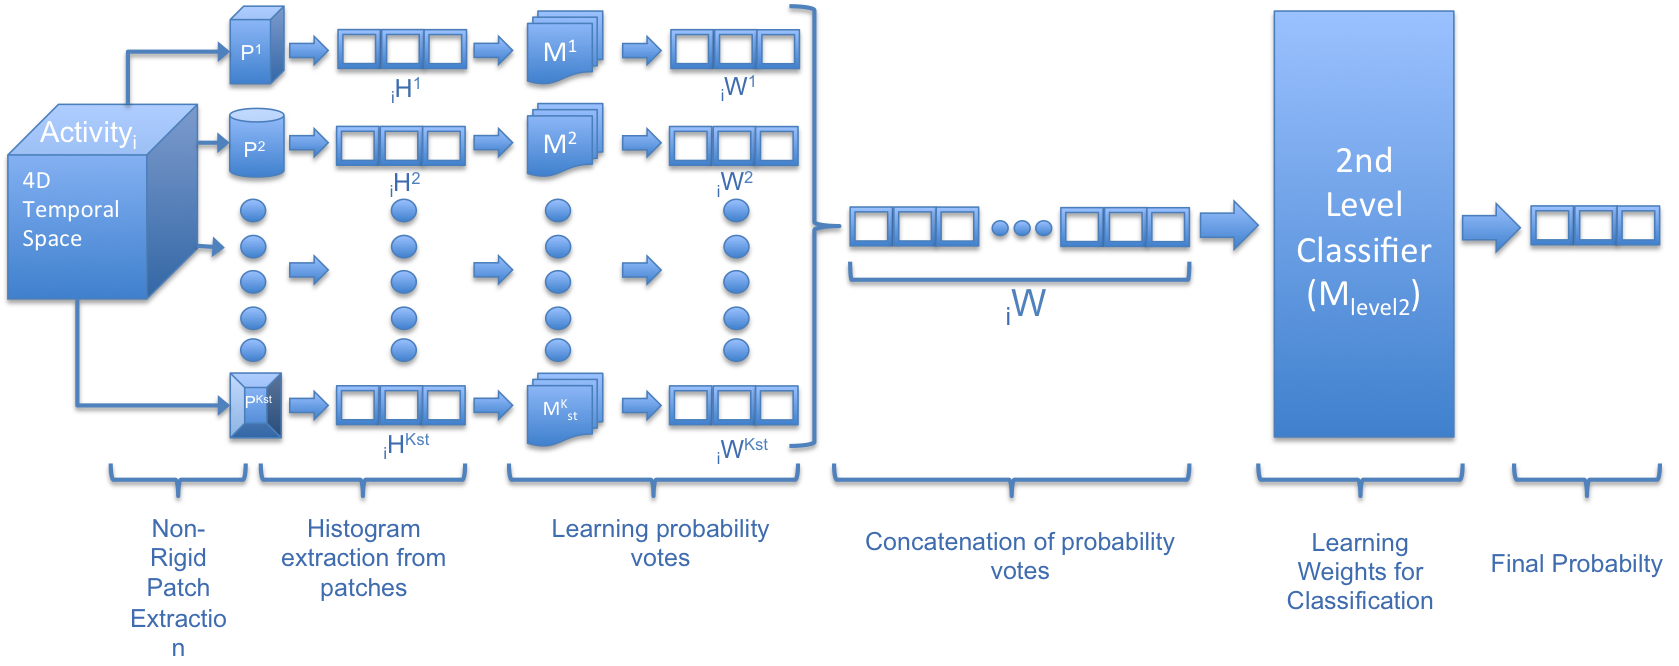
\includegraphics[scale=0.5]{Figures/multiModelApproach3}
\end{center}
\caption{Illustration of multi-model approach to classify a video clip \label{fig:multiModelApproachIllustration}}
\end{figure}





























% Chapter 4

\chapter{Experiments} % Main chapter title

\label{Chapter4} % For referencing the chapter elsewhere, use \ref{Chapter3} 

\lhead{Chapter 4. \emph{Experiments}} % This is for the header on each page - perhaps a shortened title

%----------------------------------------------------------------------------------------
In this chapter, experimental setup and results are described. First, the dataset is explained in detail with quantitative information. Then, feature extraction and encoding parameters and classification setups are shown and explained. Finally, results of evaluation of the proposed voting scheme are presented.
    
    \section{Experimental Setup}
    \label{section:ExperimentalSetup}
    
	    \subsection{Dataset}
        \label{section:Dataset}
        In order to evaluate the performance of the proposed voting scheme with data-driven 4D spatio-temporal patches, the dataset collected by \citet{twinanda2015data} is used. Composed of intensity and depth videos from 2 different views, the dataset has 11 days of recording of the operating room with real surgeries. The dataset is annotated with 15 different general and surgery-specific activities. The general activities are the common activities taking place in the operating room, e.g., bed entering, moving patient to OR bed, bed leaving, moving patient from OR bed, etc. The surgery-specific activities are picked from vertebroplasty procedures due to its frequency in the dataset. Vertebroplasty is a surgical procedure to stabilize the spinal fractures in which bone cement is injected through small punctures on the patient's skin to reduce pain. The dataset has 3 vertebroplasty specific activities, i.e., hammering, mixing cement and cement injection. It contains 1734 annotated video clips. Number of instances for each class are shown in Figure~\ref{fig:datasetChart}. Since the dataset is unbalanced as shown in Figure~\ref{fig:datasetChart}, bagging approach is used to balance instances from each class.


\begin{center}
\begin{figure}
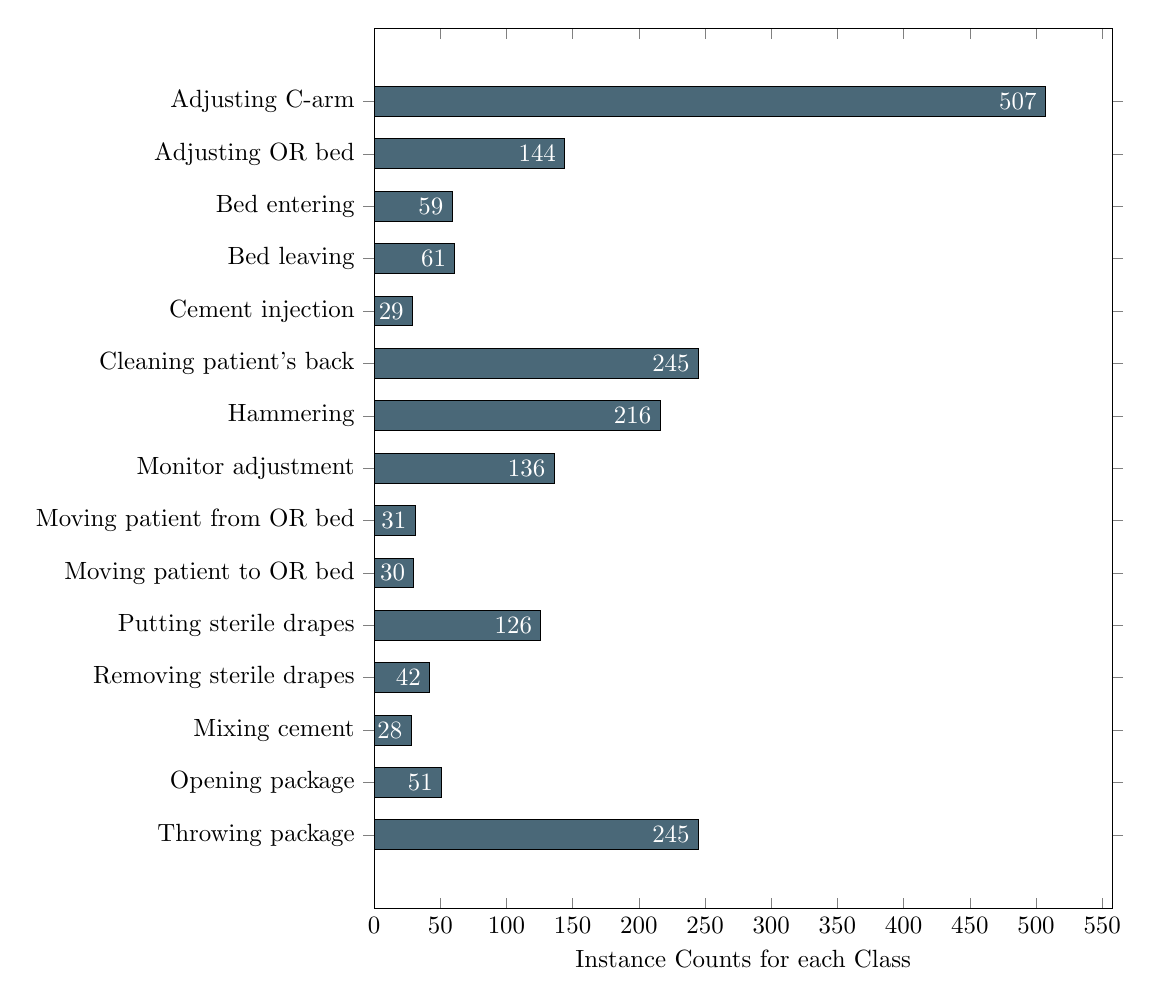
\begin{tikzpicture}[scale=0.9]
\begin{axis}[
    xbar,
    bar width=\baselineskip,
    xmin=0.0,
    width=12cm,
    height=14cm,
    ytick={1,2,3,4,5,6,7,8,9,10,11,12,13,14,15},
    yticklabels={{Throwing package},{Opening package},{Mixing cement},{Removing sterile drapes},{Putting sterile drapes},{Moving patient to OR bed},{Moving patient from OR bed},{Monitor adjustment},{Hammering},{Cleaning patient’s back},{Cement injection},{Bed leaving},{Bed entering},{Adjusting OR bed},{Adjusting C-arm}},
    enlarge y limits=0.1,
    xlabel={Instance Counts for each Class},
    ytick=data,
    nodes near coords,
    nodes near coords align=left,
    every node near coord/.style={color=white}
]
\addplot [draw=black, fill=cyan!40!black] coordinates {
    (245, 1)
    (51, 2)
    (28, 3)
    (42, 4)
    (126, 5)
    (30, 6)
    (31, 7)
    (136, 8)
    (216, 9)
    (245, 10)
    (29, 11)
    (61, 12)
    (59, 13)
    (144, 14)
    (507, 15)
};
\end{axis}
\end{tikzpicture}
\caption{Dataset Information}
\label{fig:datasetChart}
\end{figure}
\end{center}

\subsubsection{Activities in Dataset}
The dataset has 15 different activities occurs in an hybrid operating room that are shown in Figure~\ref{fig:DatasetActivities}.

\begin{itemize}
	\item \textbf{Adjusting C-Arm:} Most frequent activity in the dataset. Robotic C-Arm is moved by clinicians for taking x-ray images.
	\item \textbf{Adjusting OR Bed:} The operating room bed is moved by clinicians. 
	\item \textbf{Bed Entering:} The bed enters the operating rooms empty or with a patient.
	\item \textbf{Bed Leaving:} The bed leaves the operating room empty or with a patient.
	\item \textbf{Cement Injection:} Cement is injected to patient and during the operation operating room is dark which cause high detection in intensity data. One of the imbalance instance in dataset.
	\item \textbf{Cleaning Patient's Back:} Clinicians sterilize patient by cleaning the operation area of the patient's skin.
	\item \textbf{Hammering:} Small needle is hammered through patient's fractured vertebra with continuous x-ray captures.
	\item \textbf{Monitor or Protection Adjustment:} Clinicians adjust display monitors according to surgeons mostly before the operations. Protection equipment for x-ray beams are moved during the x-ray acquisition. 
	\item \textbf{Move Patient from OR Bed:} Patient is moved from operating room bed to portable bed after operation ends.
	\item \textbf{Move Patient to OR Bed:} After patient enters the operating room, anesthesia is applied and then the patient moved to operating room bed.
	\item \textbf{Putting Sterile Drape:} After cleaning patient's skin, sterile drapes are put to cover patient except the operating place.
	\item \textbf{Removing Sterile Drape:} After operation is ended, clinicians remove the sterile drapes and throw them to thrash.
	\item \textbf{Mixing Cement:} Cement is mixed by surgeon before cement injection procedure. Most Vertoblasty operations have one mixing cement activity. Mixing cement is the most imbalanced instance in our dataset.
	\item \textbf{Opening Package:} Packages that contain operation tools get opened on operating room tool table.
	\item \textbf{Throwing Package:} After operation ends, clinicians throw packages on the tool table to trash.
\end{itemize}

\begin{figure}[!htbp]
\centering
\subfigure[Adjusting C-Arm]{\label{sfig:a}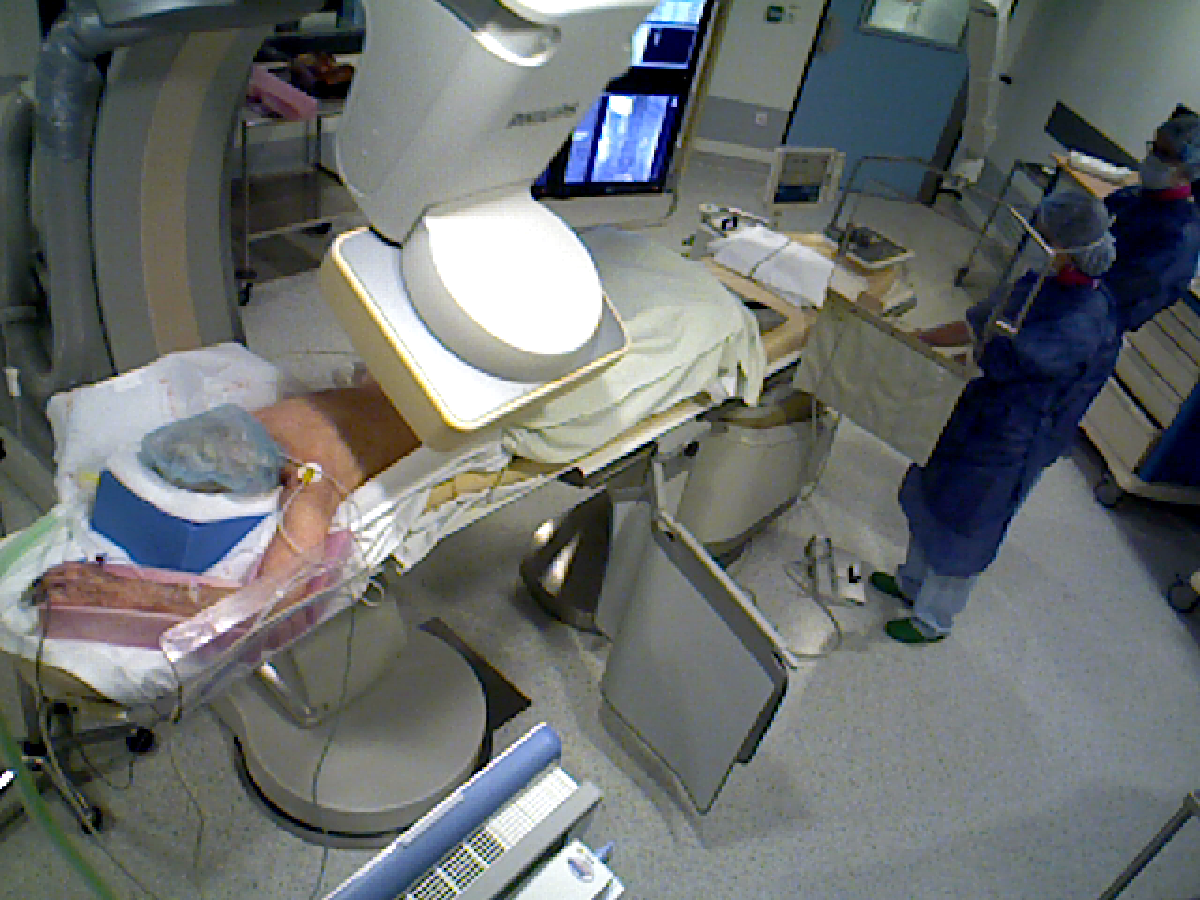
\includegraphics[width=.33\textwidth]{Figures/Actions/01_AdjustingCArm}}\hfill
\subfigure[Adjusting OR Bed]{\label{sfig:b}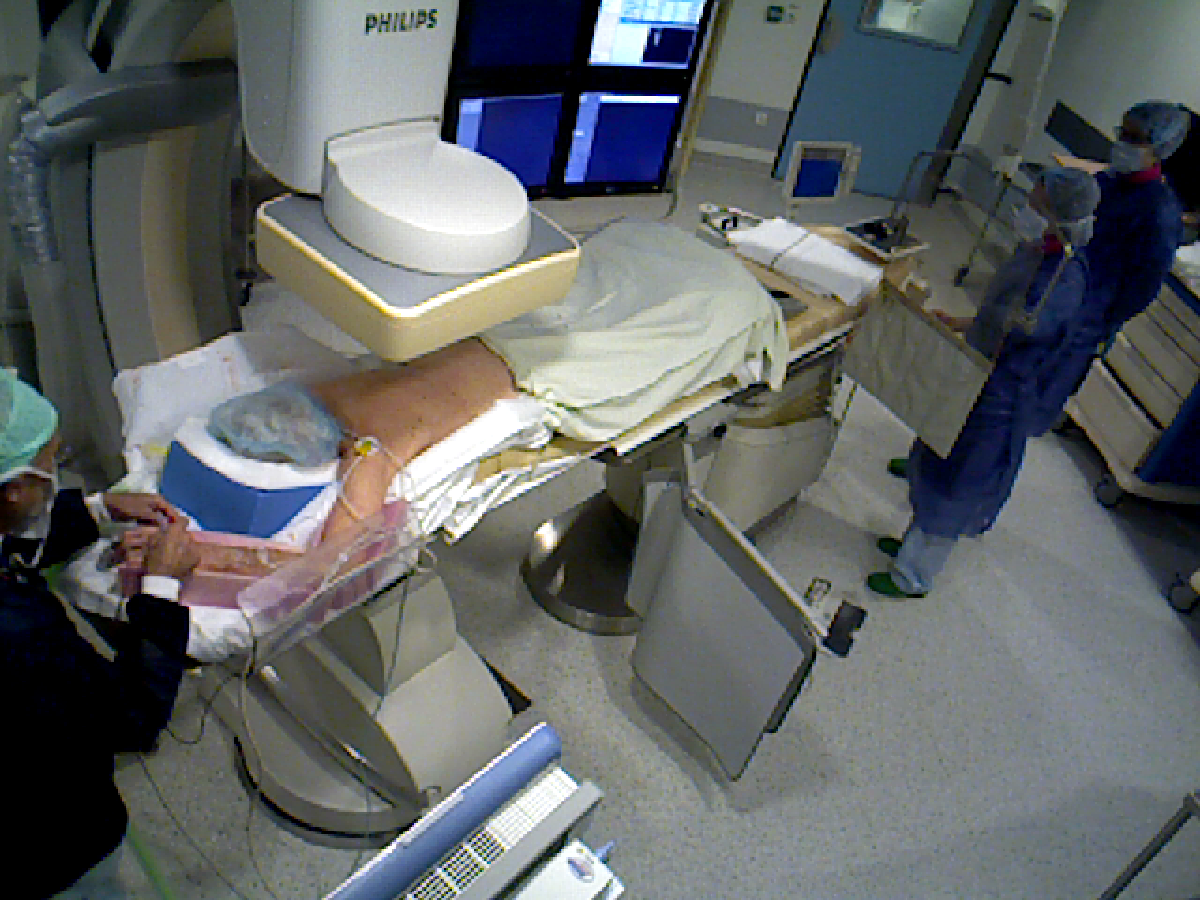
\includegraphics[width=.33\textwidth]{Figures/Actions/02_AdjustingORBed}}\hfill
\subfigure[Bed Entering] {\label{sfig:c}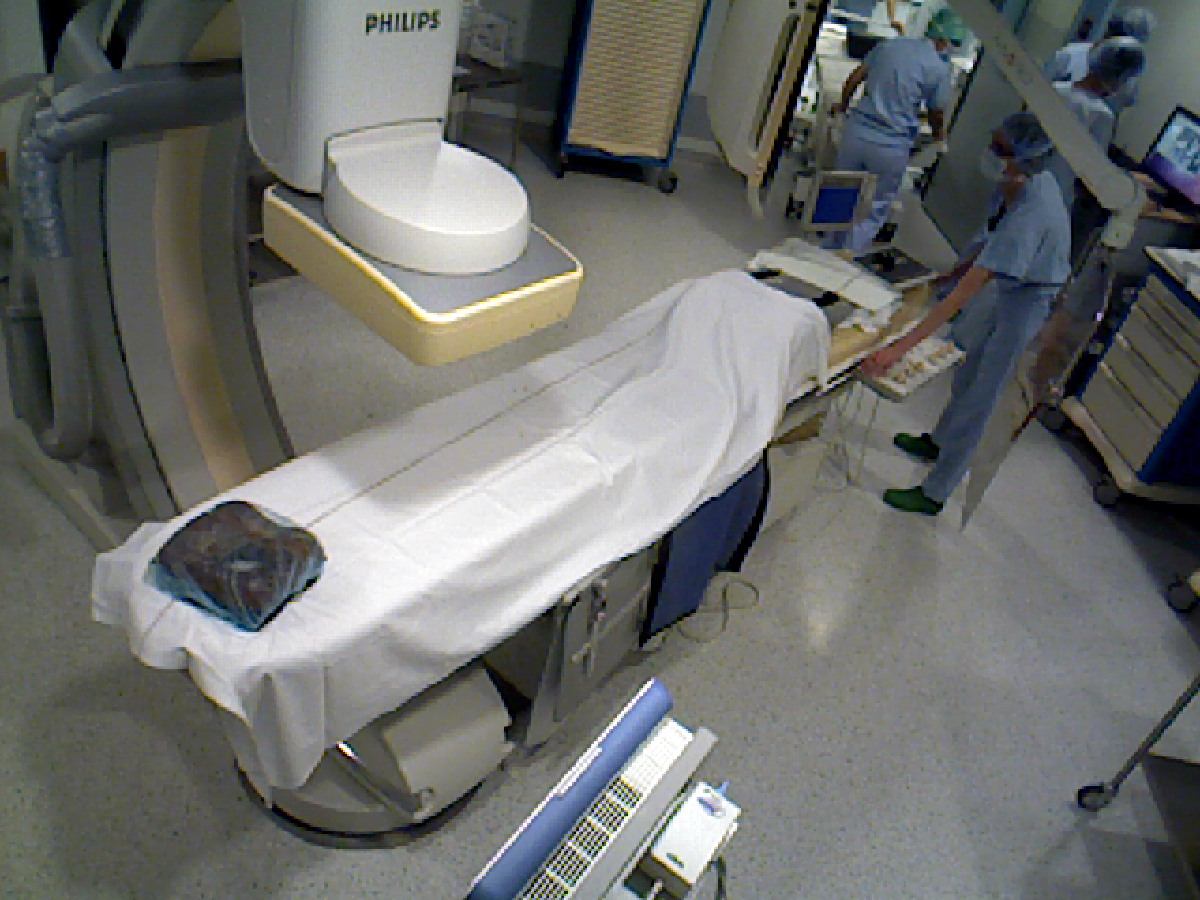
\includegraphics[width=.33\textwidth]{Figures/Actions/03_BedEntering}}\\
\subfigure[Bed Leaving]{\label{sfig:d}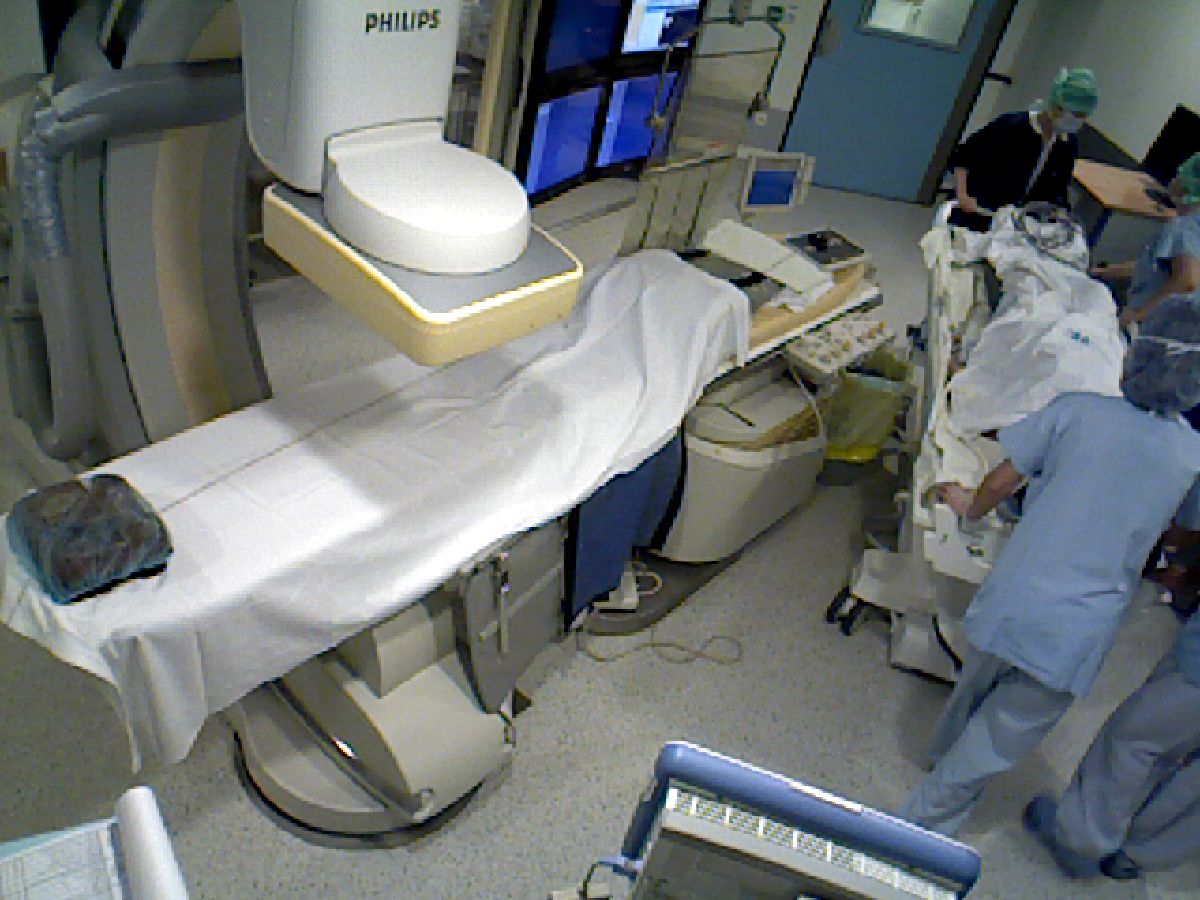
\includegraphics[width=.33\textwidth]{Figures/Actions/04_BedLeaving}}\hfill
\subfigure[Cement Injection]{\label{sfig:e}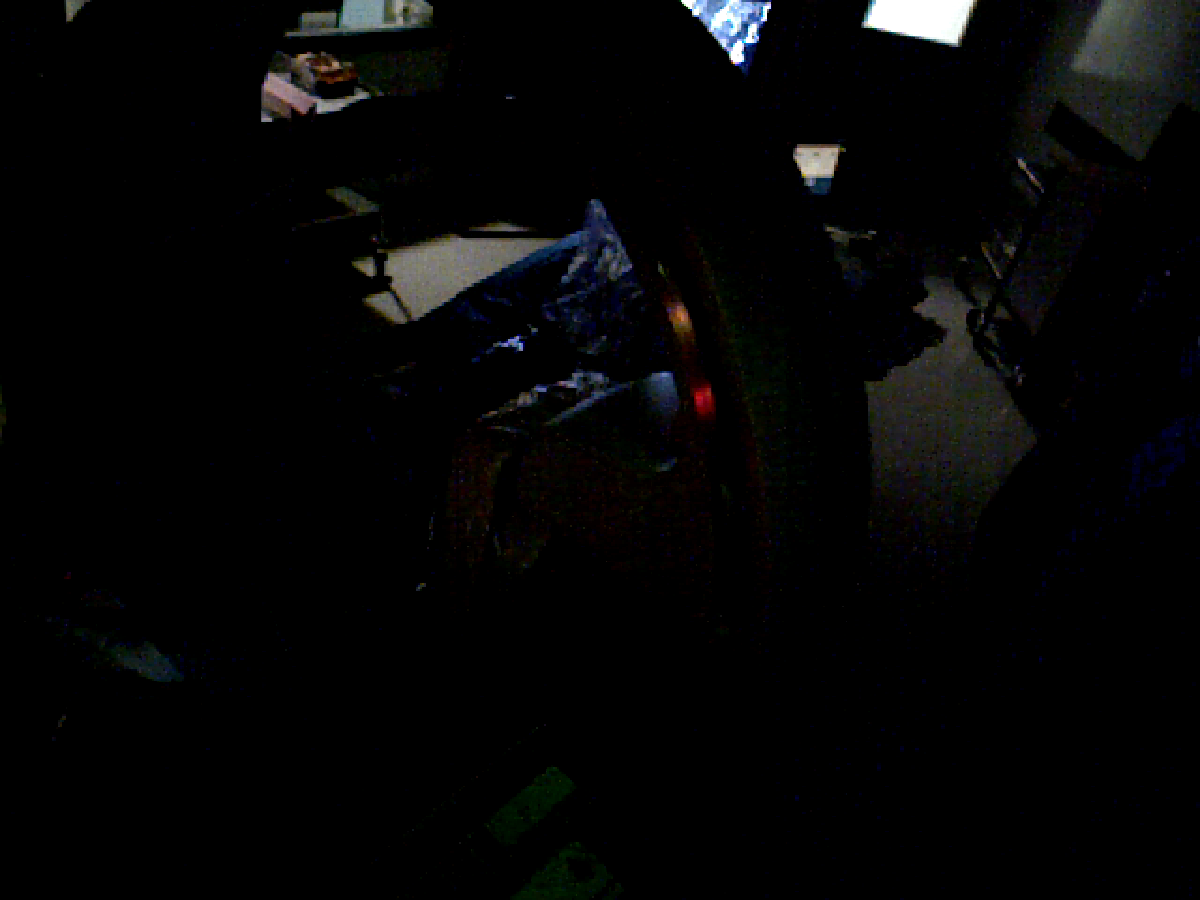
\includegraphics[width=.33\textwidth]{Figures/Actions/05_CementInjection}}\hfill
\subfigure[Cleaning Patient's Back]{\label{sfig:f}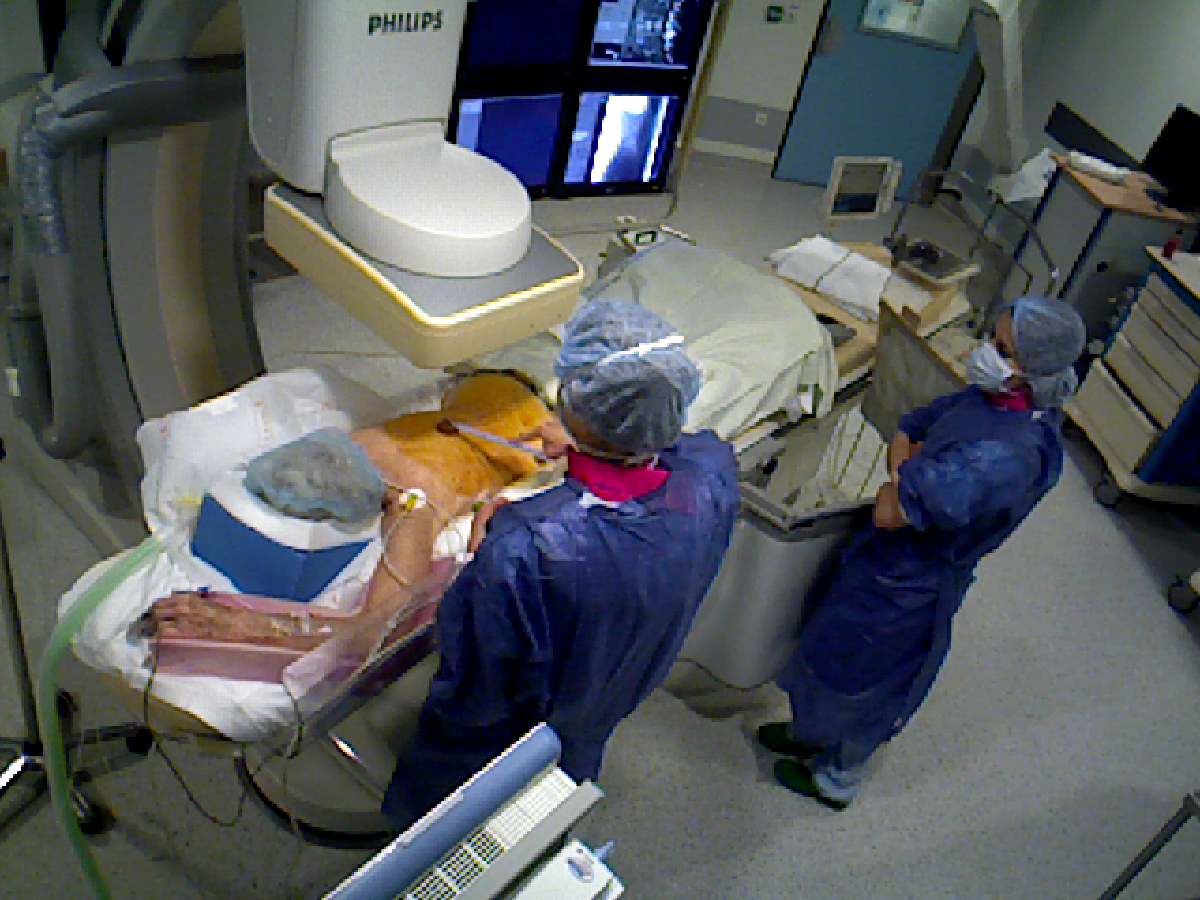
\includegraphics[width=.33\textwidth]{Figures/Actions/06_CleaningPatientBack}}\\
\subfigure[Hammering]{\label{sfig:g}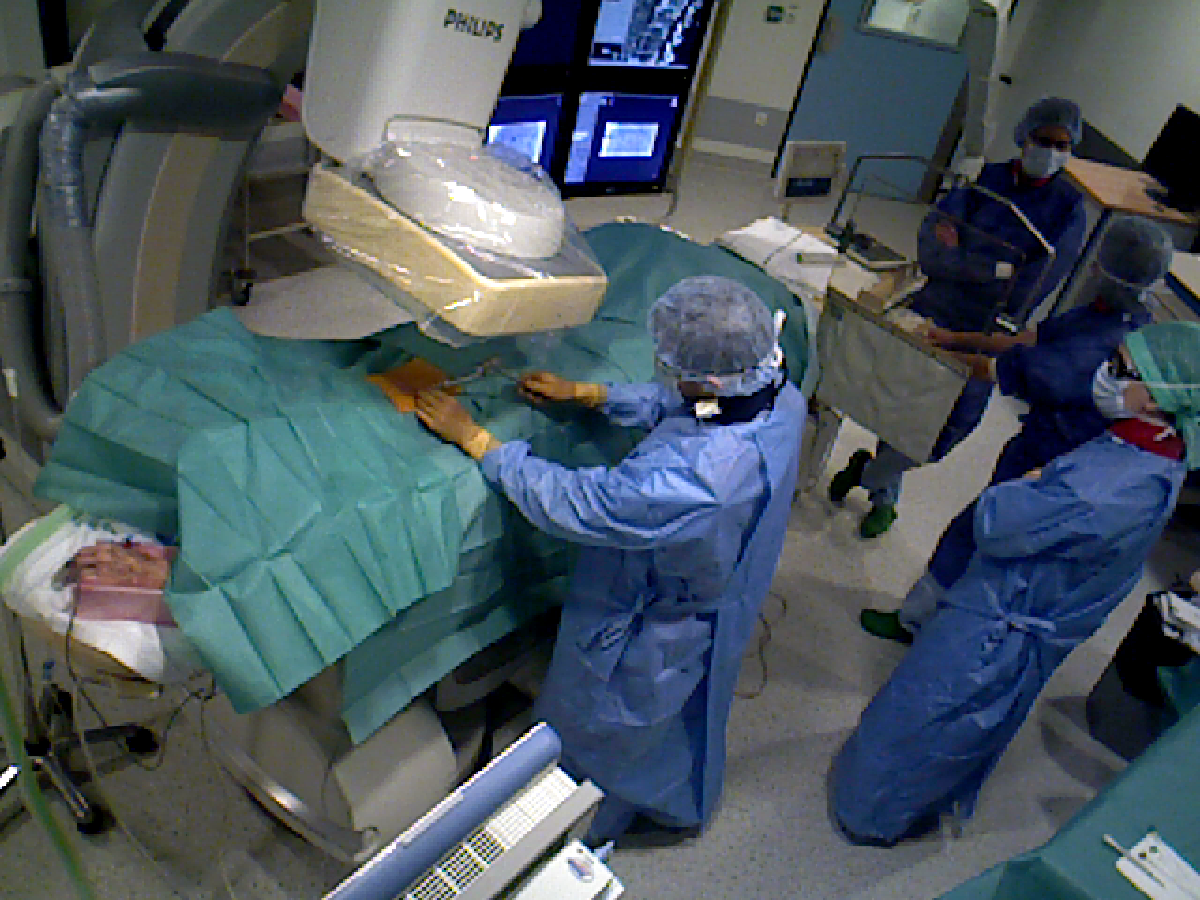
\includegraphics[width=.33\textwidth]{Figures/Actions/07_Hammering}}\hfill
\subfigure[Monitor or Protection Adjustment]{\label{sfig:h}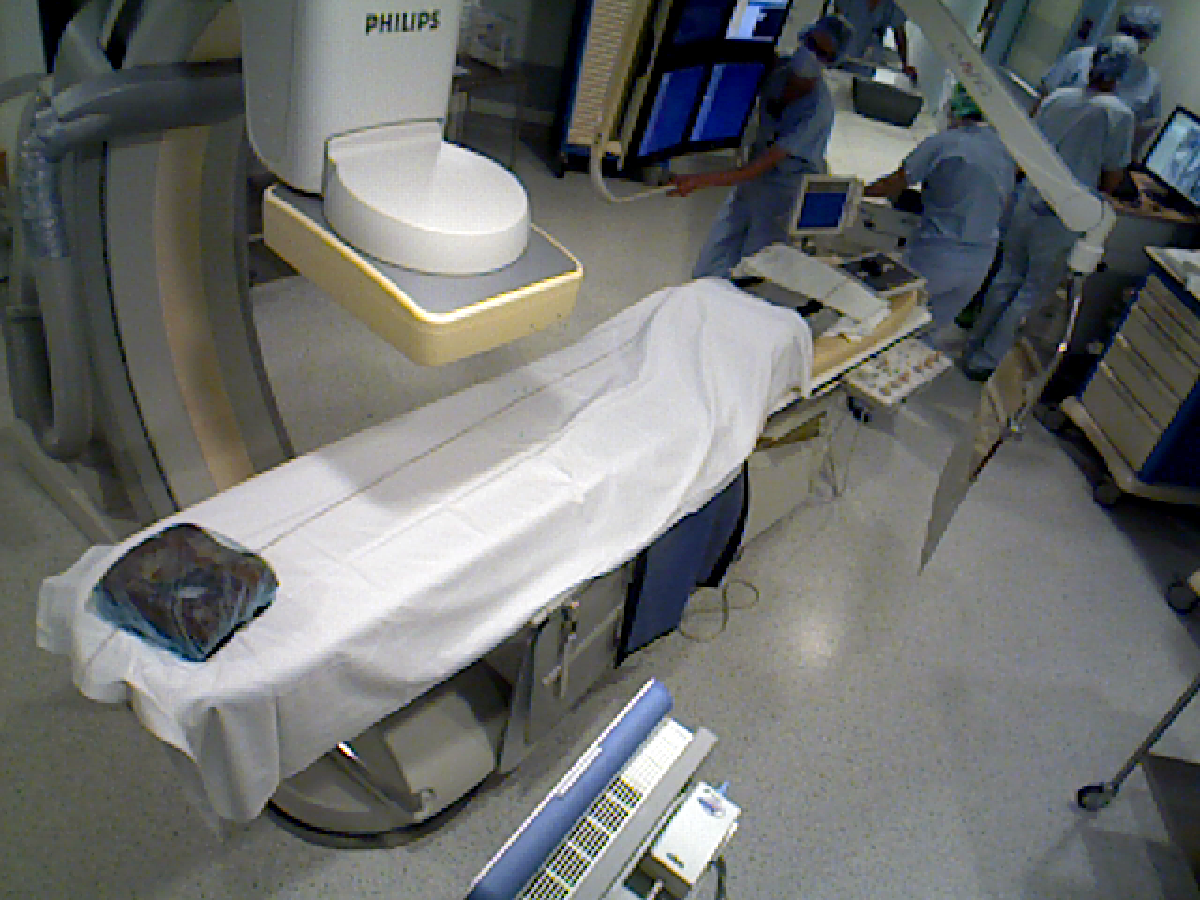
\includegraphics[width=.33\textwidth]{Figures/Actions/08_MonitorAdjustment}}\hfill
\subfigure[Move Patient from OR Bed]{\label{sfig:i}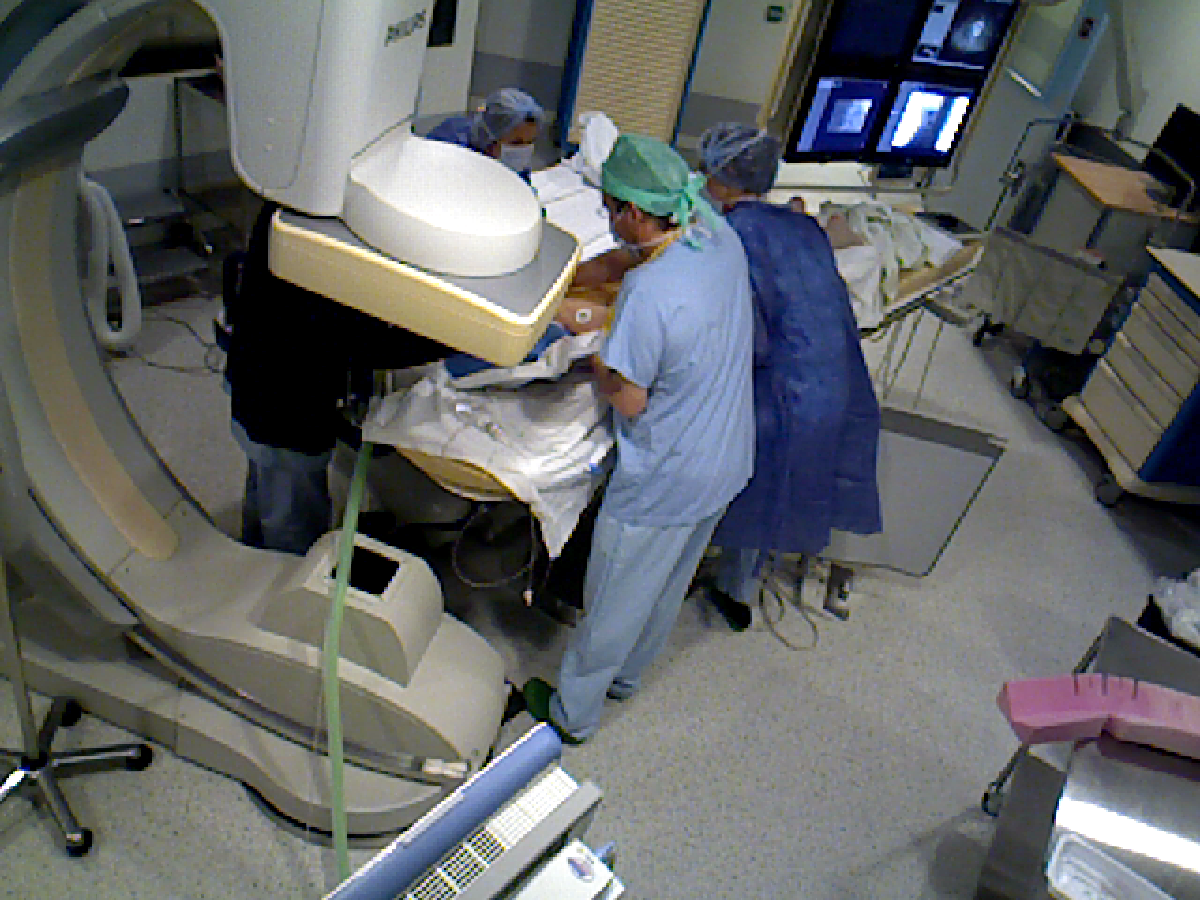
\includegraphics[width=.33\textwidth]{Figures/Actions/09_MovePatientFromORBed}}\\
\subfigure[Move Patient to OR Bed]{\label{sfig:j}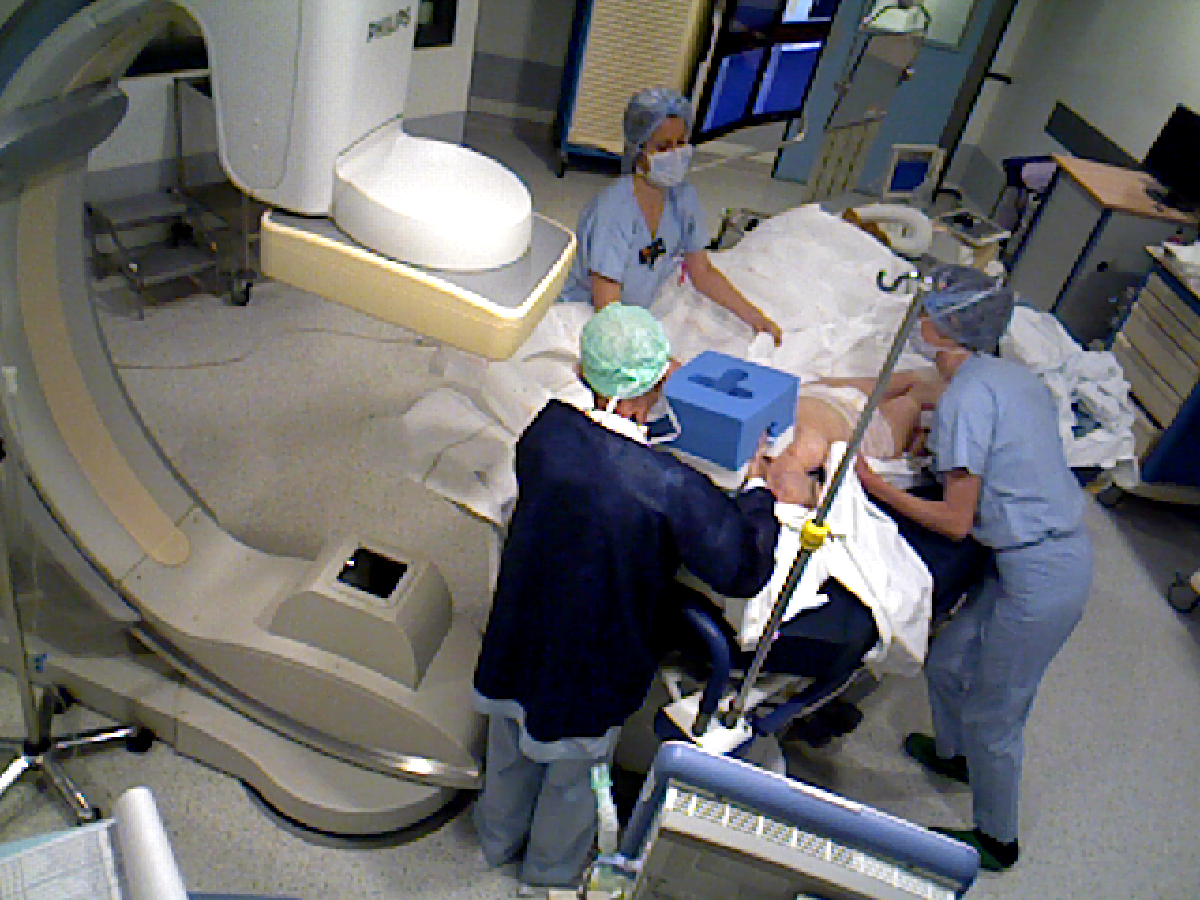
\includegraphics[width=.33\textwidth]{Figures/Actions/10_MovePatientToORBed}}\hfill
\subfigure[Putting Sterile Drape]{\label{sfig:k}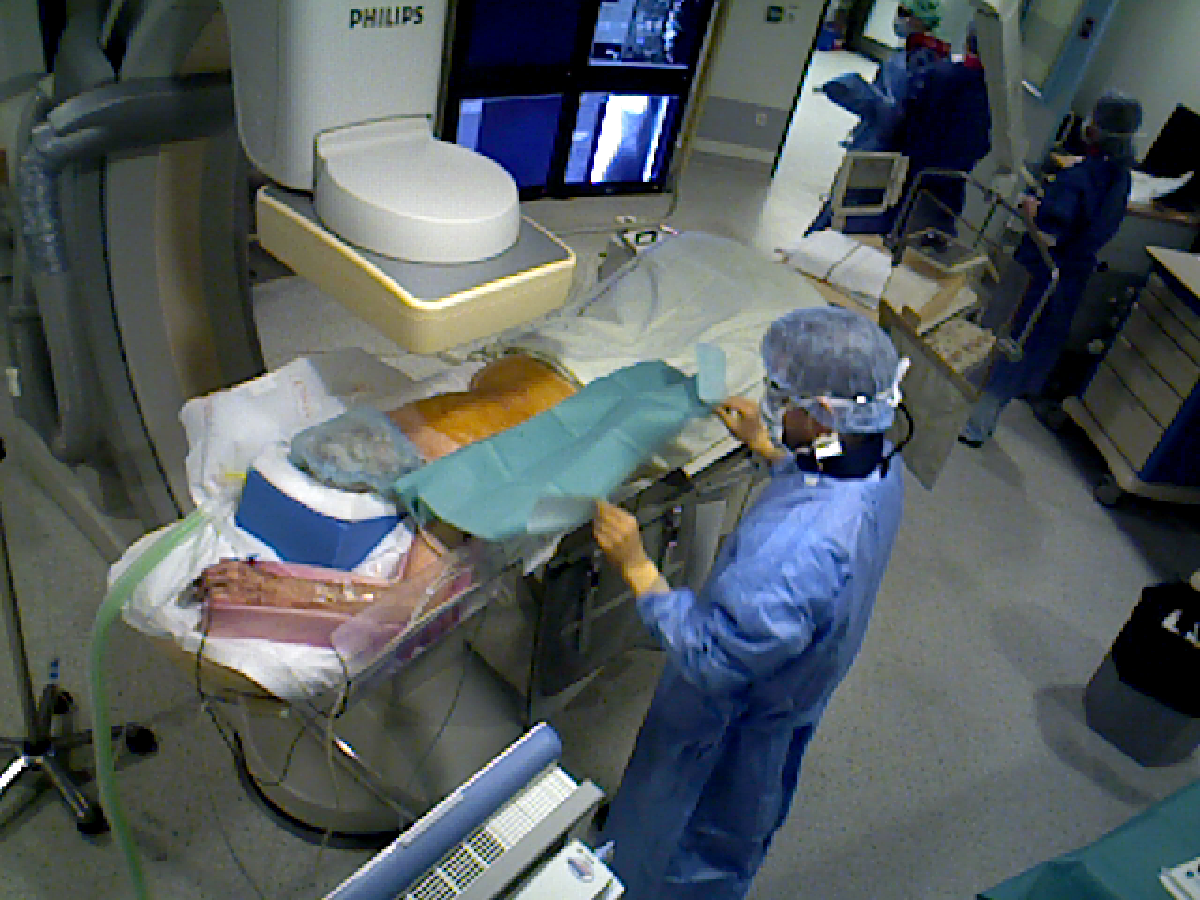
\includegraphics[width=.33\textwidth]{Figures/Actions/11_PuttingSterileDrape}}\hfill
\subfigure[Removing Sterile Drape]{\label{sfig:l}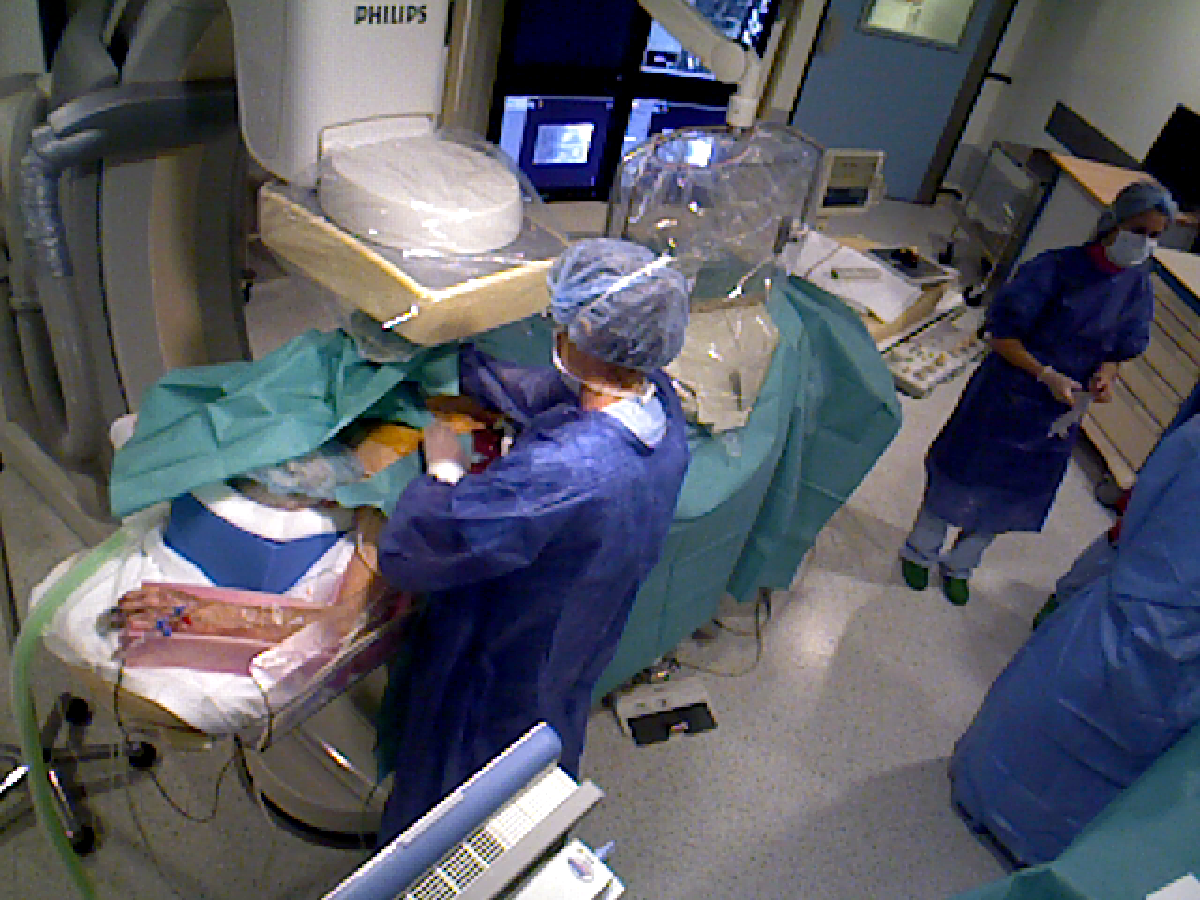
\includegraphics[width=.33\textwidth]{Figures/Actions/12_RemovingSterileDrape}}\\
\subfigure[Mixing Cement]{\label{sfig:m}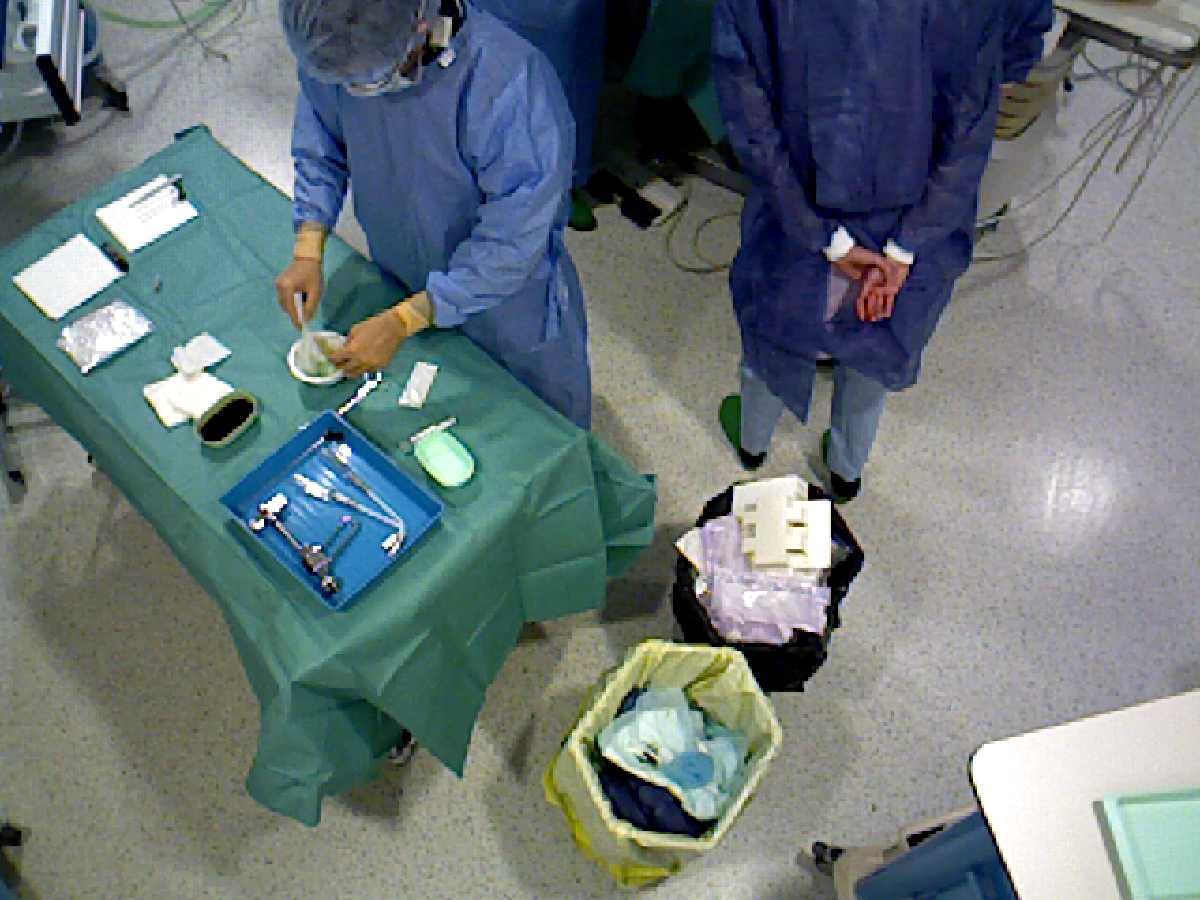
\includegraphics[width=.33\textwidth]{Figures/Actions/13_MixingCement}}\hfill
\subfigure[OpeningPackage]{\label{sfig:n}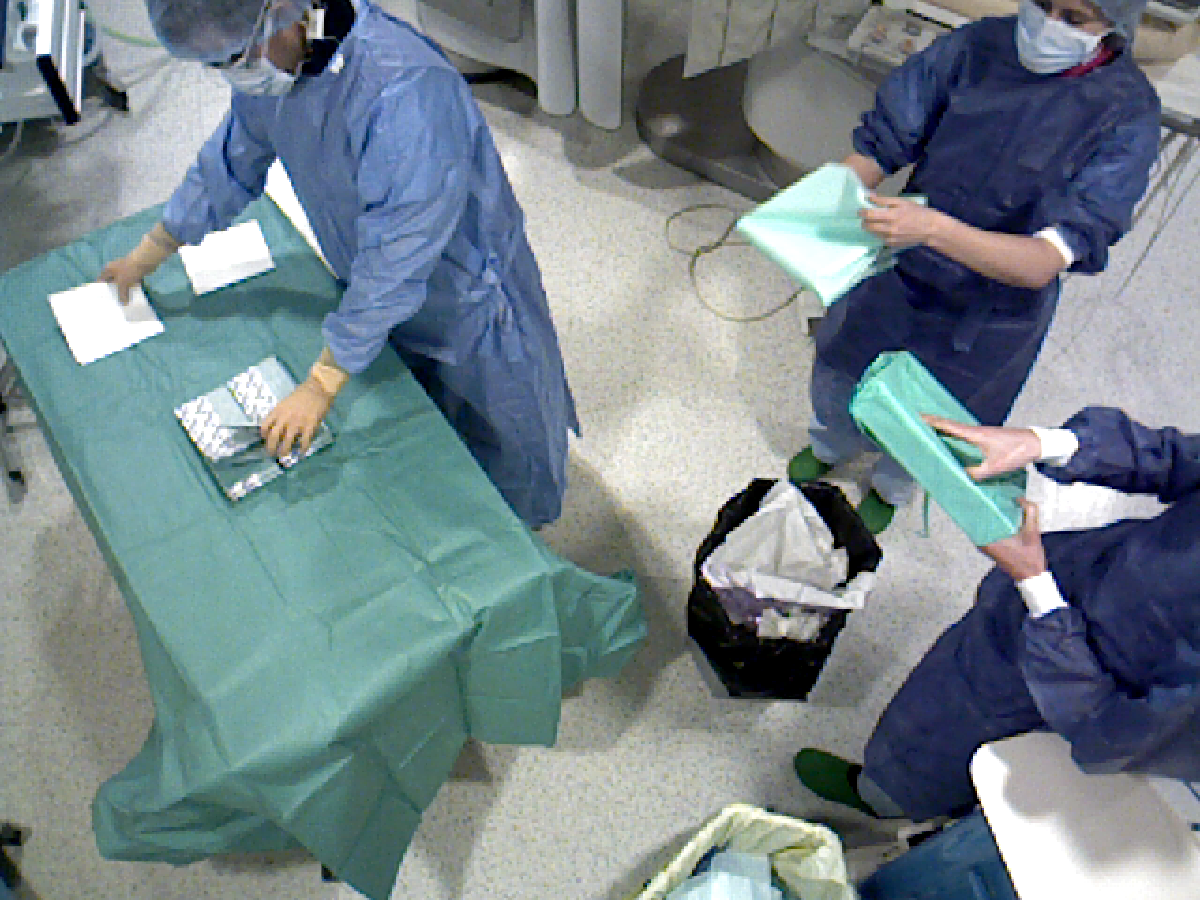
\includegraphics[width=.33\textwidth]{Figures/Actions/14_OpeningPackage}}\hfill
\subfigure[Throwing Package]{\label{sfig:o}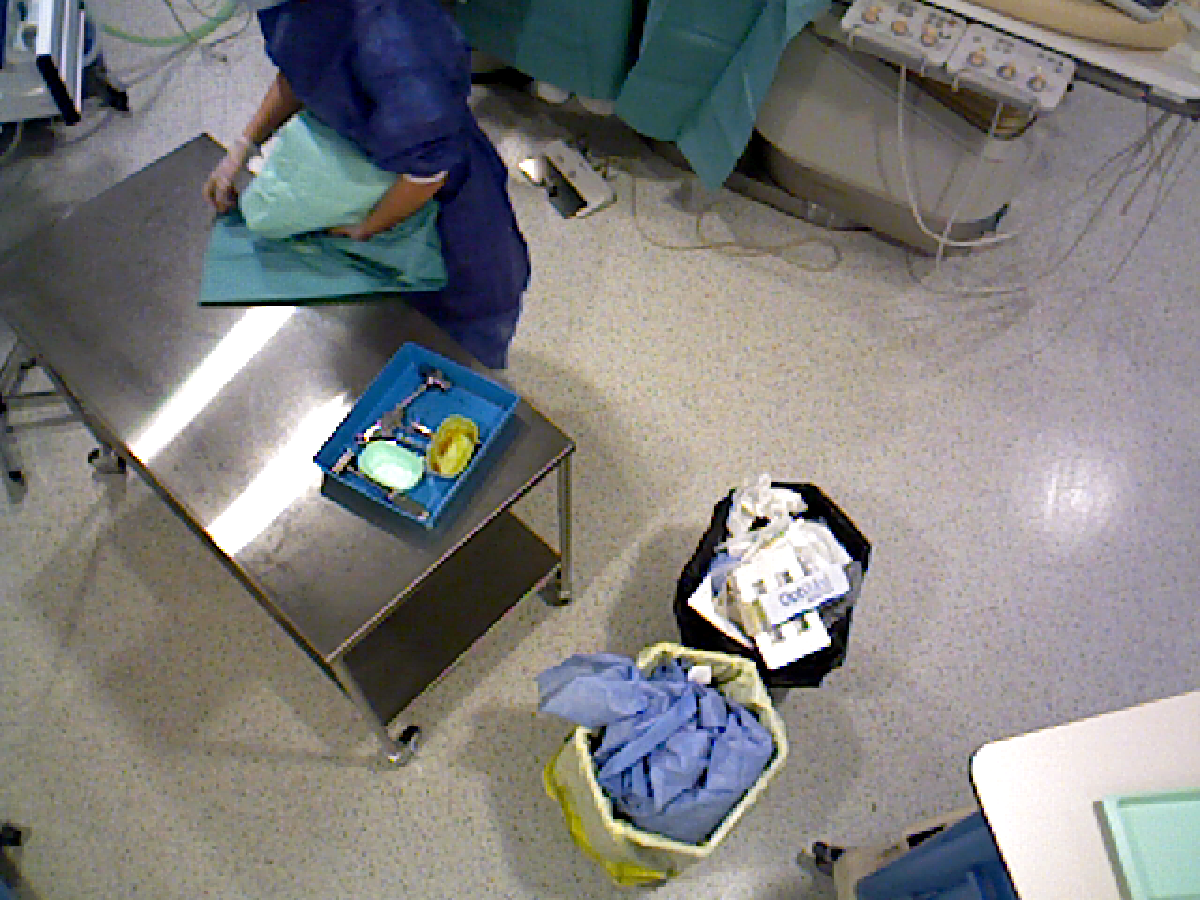
\includegraphics[width=.33\textwidth]{Figures/Actions/15_ThrowingPackage}}\\

\caption{Activity types in the dataset - samples of intensity images}
\label{fig:DatasetActivities}
\end{figure}
    
    	\subsection{Visual feature extraction and encoding}
        \label{section:VisualFeatureExtractionAndEncoding}
        In interest point detection, we detect 1000 STIPs from intensity and 1000 DSTIPs from depth data from each video clip. Then, we extract 480-dimensional HOF from intensity and 4005-dimensional DCSF from depth data around each interest point. We use Principal Component Analysis (PCA) to reduce dimensions of HOF and DSCF to 250 and 800 respectively for visual dictionary construction. All these parameters have proven to produce good results in \citet{twinanda2015data}. In \cite{twinanda2015data}, performance comparison of size of visual dictionaries are studied and it is shown that visual dictionary size 1500 has the highest accuracy and increasing the number of words in dictionary size has not much improve the performance. Then second dictionary, spatio-temporal dictionary, is built to divide 4D spatio-temporal space into non-rigid cells with 24 patches for intensity and depth data. When we use combination of intensity and depth data, the number of 4D patches becomes 48 (24 from both intensity and depth).

        
        \subsection{Classification Setup}
        \label{section:ClassificationStrategy}
        In this work, we use Support Vector Machine (SVM) and Random Forest (RF) classifiers. In the experiments, two-level classification strategy is used and explained in detail in Section~\ref{section:TrainingStrategy}. We also use two different approaches: one-model and multi-model. In one-model approach, a single classifier model is trained on each level. In contrast, in the multi-model approach, multiple classifier models are trained on the first level. For intensity and depth data, 24 classifier models are trained. However, for the combination, 48 classifier models are trained. These numbers are used to match the number of 4D patches.
        
        
        \subsubsection{SVM Setup}
        \label{section:SVMSetup}
         SVM models in the experiments are trained using VLFeat toolbox \cite{Vedaldi:2010:VOP:1873951.1874249}. SVM is used with non-linear kernels, i.e., Chi-square $ \left(\mathcal{X}\right)^{2} $ and histogram intersection kernels. Since there is 15 different classes for classification, one-against-all SVM is used to handle multi-class problem. K-Fold cross validation is used to evaluate performance by dividing the dataset into 10 folds.
        
        \subsubsection{Random Forest Setup}
        \label{section:RandomForestSetup}
        Random Forest models in the experiments are trained using our own implementation of Random Forest. Random Forests depend on many parameters, e.g., number of trees, maximum depth of the trees, minimum information gain and minimum number of samples in each tree node as stopping criteria to stop building a tree. Random Forests are trained with 100 trees, with maximum depth 15. The minimum information gain in the node is set to 0.001 to avoid trees with low information gain. One of the effective parameter in tree building is the minimum number of samples reach to each node before stopping. We use 32 samples as minimum number of samples in node as stopping criteria. Each tree in the random forest have seen 80\% of the training data as randomly for bagging across trees. Finally K-Fold cross validation is used to evaluate the performance by dividing the dataset into 10 folds.


\section{Experimental Results}
\label{section:ExperimentalResults}

In this section, we report results from the voting scheme as well as the comparison with non-voting scheme. We also compare the one-model and multi-model approaches using the proposed two-level classification strategy with the voting scheme, and their results compared on intensity, depth and the combination of the intensity and depth.

%     In this section, we conduct experiments to verify and evaluate our proposed voting scheme strategy on the aforementioned dataset \cite{twinanda2015data} and report the results by comparing to non-voting approach \cite{twinanda2015data}. We use intensity, depth and their combination individually for evaluation using two different classifiers, i.e., non-linear SVM and Random Forest. In the experiments we use two different evaluation methods that changes classification strategy: one-model and multi-model strategies that their setup is described in Section~\ref{ClassificationStrategy}. We share results from the one model and multi model under Section~\ref{section:OneModel} and Section~\ref{section:MultiModel} respectively.
    
\subsection{One Model Approach}
\label{section:OneModelExperiments}
In the one-model approach, we learn a single SVM and Random Forest model in each level with all patches from each activity. In Table~\ref{table:oneModelResults}, results for one-model approach is presented with intensity, depth and combination of the data with both of the classifiers. It is shown that non-linear SVM performs slightly better than the Random Forest. It is also shown that combination of the intensity and depth data has more discriminating power than using only intensity or depth. The combination of the depth and intensity profits the complementary information that intensity and depth carries. Because some activities are well classified in intensity due to illumination and intensity changes, e.g., cement injection, however some actions showed better performance in depth due to high variance in depth, e.g., Adjusting C-Arm. These effects are shown in confusion matrices in Figure~\ref{fig:intensityOneModelConfusionMatrix} and Figure~\ref{fig:depthOneModelConfusionMatrix}. The combination of the intensity and depth data gets the highest accuracy with 83.1\% accuracy using SVM and the confusion matrix is shown in Table~\ref{fig:combinationOneModelConfusionMatrix}.


\begin{table}[h]
\centering
\begin{tabular}{|c|c|c|}
\hline
                     & \textbf{SVM}     & \textbf{RF} \\ \hline
\textbf{Intensity}   & \textbf{74.45\%} & 70.06\%     \\ \hline
\textbf{Depth}       & \textbf{72.72\%} & 67.87\%     \\ \hline
\textbf{Combination} & \textbf{83.1\%}  & 79.18\%     \\ \hline
\end{tabular}
\caption{Classification results using one-model approach}
\label{table:oneModelResults}
\end{table}

\begin{figure}[H]
\begin{center}
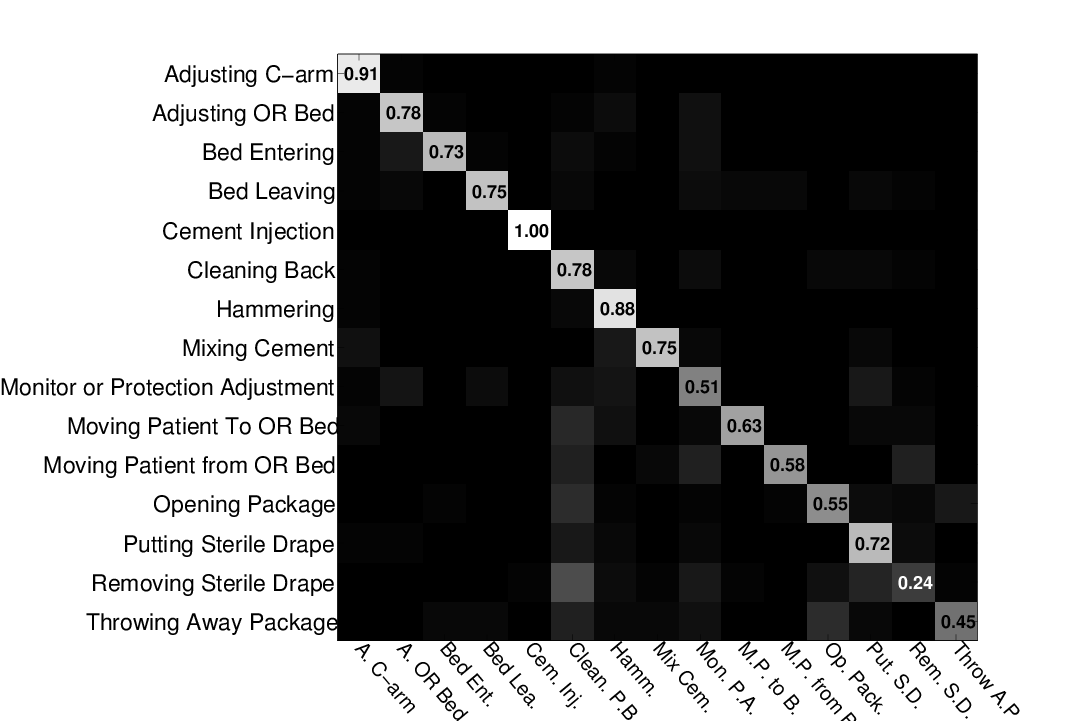
\includegraphics[scale=0.4]{Figures/intensity-onemodel}
\end{center}
\caption{Confusion matrix of one-model approach using intensity features \label{fig:intensityOneModelConfusionMatrix}}
\end{figure}
        
\begin{figure}[H]
\begin{center}
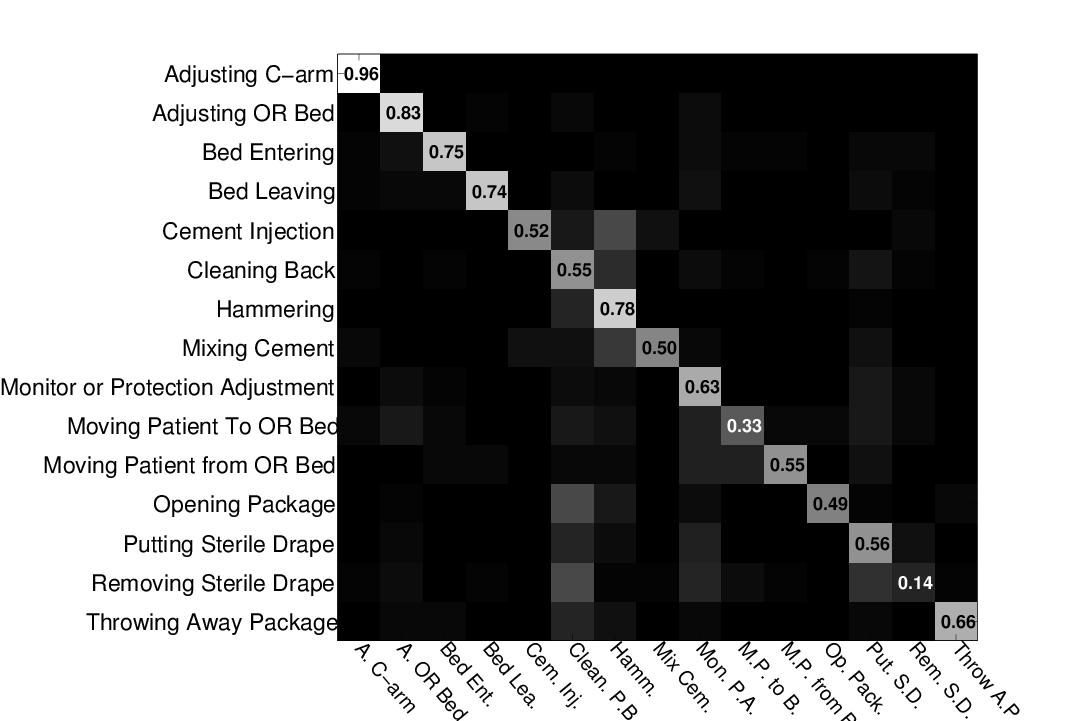
\includegraphics[scale=0.4]{Figures/depth-onemodel}
\end{center}
\caption{Confusion matrix of one-model approach using depth features \label{fig:depthOneModelConfusionMatrix}}
\end{figure}

\begin{figure}[H]%[!htbp]%[here][H]
\begin{center}
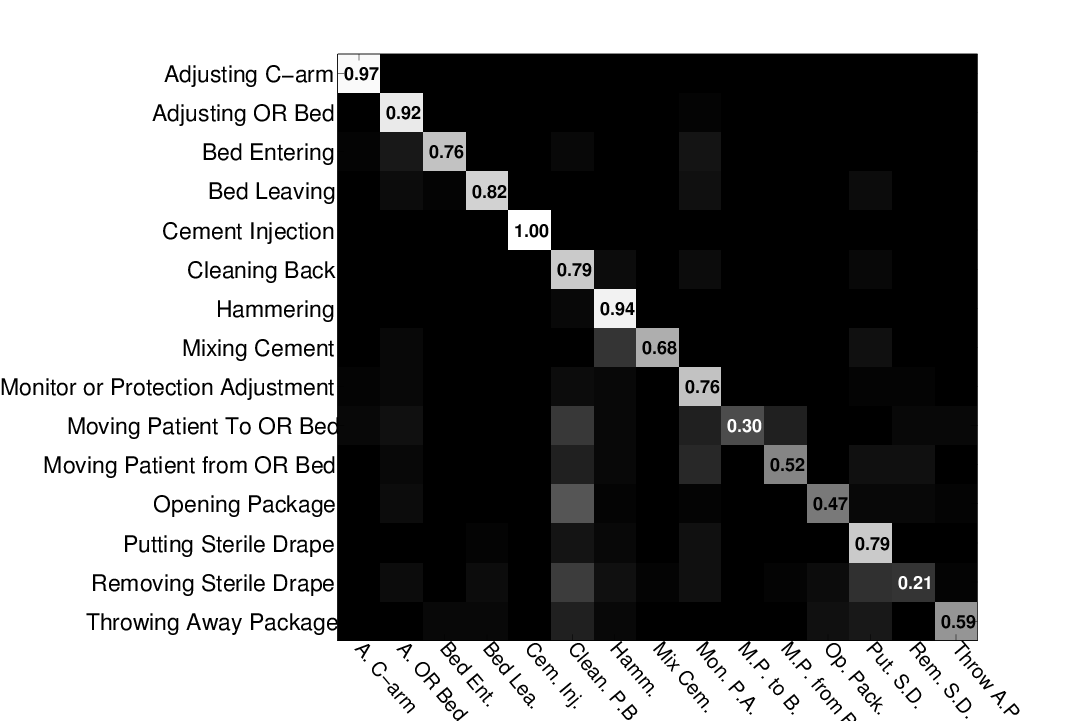
\includegraphics[scale=0.4]{Figures/combination-onemodel}
\end{center}
\caption{Confusion matrix of one-model approach using combination of features
\label{fig:combinationOneModelConfusionMatrix}}
\end{figure}

\subsection{Multi-Model}
\label{section:MultiModelExperiments}
In the multi-model approach, we learn multiple models in the first level for each patch type $P^{j}$. However, the one-model approach in Section~\ref{section:OneModelExperiments} trained a single model for the first level using all the patches from all the video clips.
Hence, one-model approach profits from seeing more training data whereas in the multi-model approach, the first level classifiers sees less training data. Thus, multi-model has slight disadvantage over one-model approach due to training the each patch model. Thus, results presented in Table~\ref{table:multiModelResults} have slighly lesser accuracy than one model results in Table~\ref{table:oneModelResults}. On the other hand, the combination of intensity and depth is still performing better than using only intensity or depth. We achieved 81.71\% accuracy with combination of the data with the SVM classifier. The detailed results are presented with confusion matrices in Figure~\ref{fig:intensityMultiModelConfusionMatrix}, \ref{fig:depthMultiModelConfusionMatrix} and \ref{fig:combinationMultiModelConfusionMatrix}.
            
\begin{table}[H]
\centering
\begin{tabular}{|c|c|c|}
\hline
                     & \textbf{SVM}     & \textbf{RF} \\ \hline
\textbf{Intensity}   & \textbf{77.28\%} & 69.20\%     \\ \hline
\textbf{Depth}       & \textbf{71.91\%} & 64.45\%     \\ \hline
\textbf{Combination} & \textbf{81.71\%} & 75.54\%     \\ \hline
\end{tabular}
\caption{Classification results using multi-model approach}
\label{table:multiModelResults}
\end{table}

\begin{figure}[H]
\begin{center}
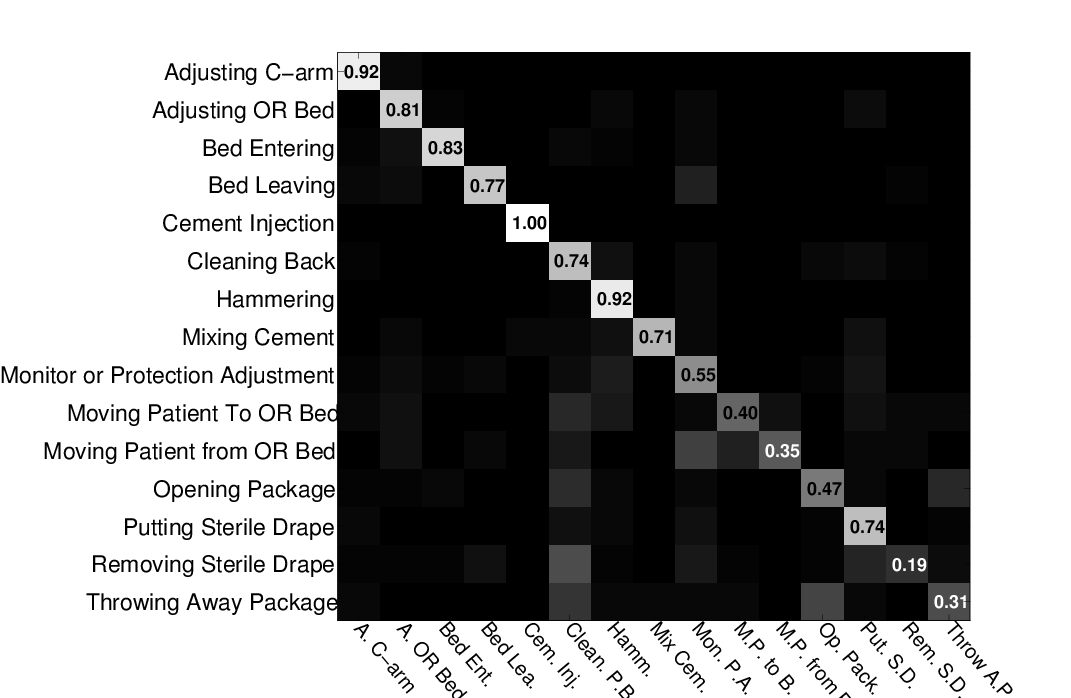
\includegraphics[scale=0.4]{Figures/intensity-multimodel}
\end{center}
\caption{Confusion matrix of multi-model approach using intensity features 
\label{fig:intensityMultiModelConfusionMatrix}}
\end{figure}
        
\begin{figure}[H]
\begin{center}
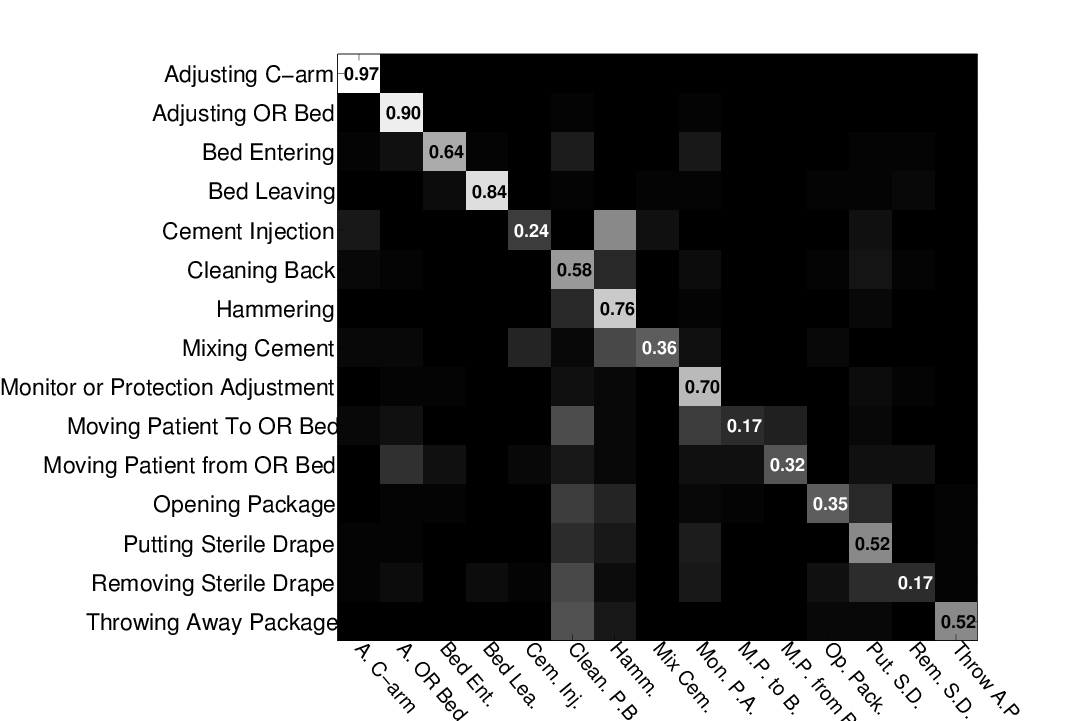
\includegraphics[scale=0.4]{Figures/depth-multimodel}
\end{center}
\caption{Confusion matrix of multi-model approach using depth features  
\label{fig:depthMultiModelConfusionMatrix}}
\end{figure}

\begin{figure}[H]%[!htbp]%[here][H]
\begin{center}
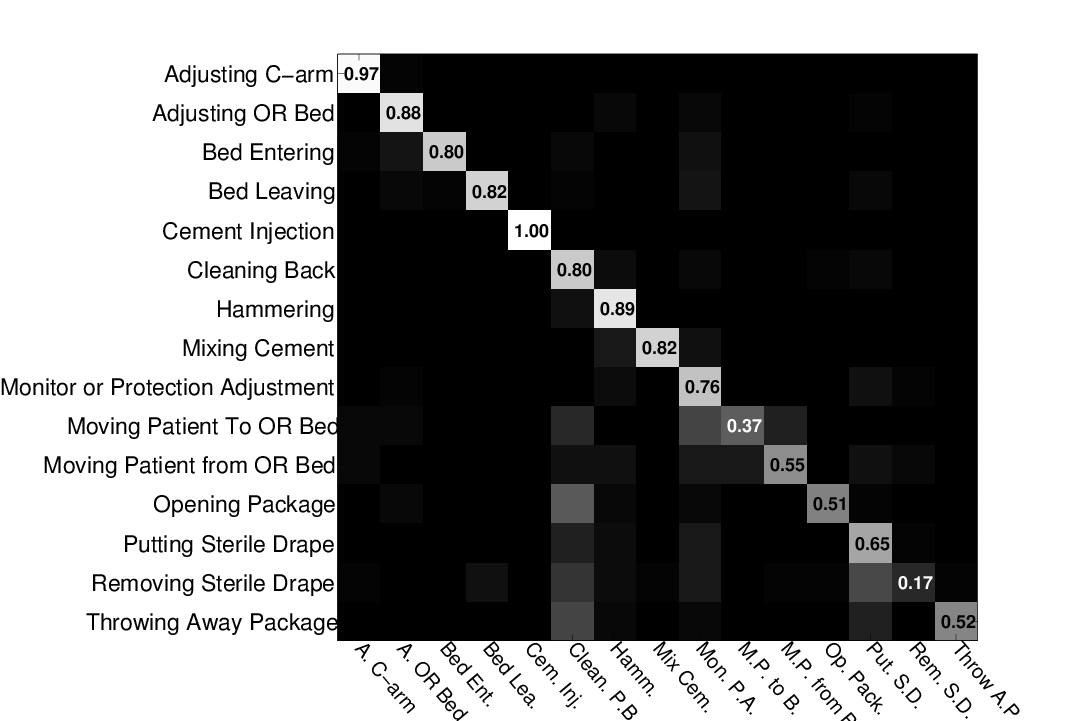
\includegraphics[scale=0.4]{Figures/comb-multimodel}
\end{center}
\caption{Confusion matrix of multi-model approach using combination of features  
\label{fig:combinationMultiModelConfusionMatrix}}
\end{figure}
            
            
            
\subsection{Non-Voting Approach}
\label{section:NonVotingAproachExperiments}
	The proposed voting scheme approach also compared to non-voting scheme approach in \cite{twinanda2015data}. In \cite{twinanda2015data}, a data-driven non-rigid layout is used by concatenating the histogram vectors from patches to construct single histogram vector to represent video clip. The histogram vector also concatenated with a histogram vector extracted from video clip without using any layout. Hence, the final concatenated histogram carries more information than using histograms from each patch separately as in Section~\ref{section:OneModelExperiments} and Section~\ref{section:MultiModelExperiments}. Using the patch histograms separately for training and collecting votes increased the sparsity problem in classification in the first level. The non-voting method reached 85.53\% accuracy compared to our maximum accuracy 83.1\%. The detailed comparison with intensity, depth data and their combination is shown in Table~\ref{table:comparisonResults}.
    
    
\begin{table}[H]
\centering
\begin{tabular}{|c|c|c|}
\hline
                  & {\bf Non-Voting \cite{twinanda2015data}}   & {\bf Voting} \\ \hline
{\bf Intensity}   & {\bf 80.40\%} & 74.45\%    \\ \hline
{\bf Depth}       & {\bf 78.37\%} & 72.72\%    \\ \hline
{\bf Combination} & {\bf 85.53\%} & 83.1\%     \\ \hline
\end{tabular}
\caption{Classification accuracy comparison of non-voting \cite{twinanda2015data} and voting scheme}
\label{table:comparisonResults}
\end{table}
           


\begin{figure}[H]%[!htbp]%[here][H]
\begin{center}
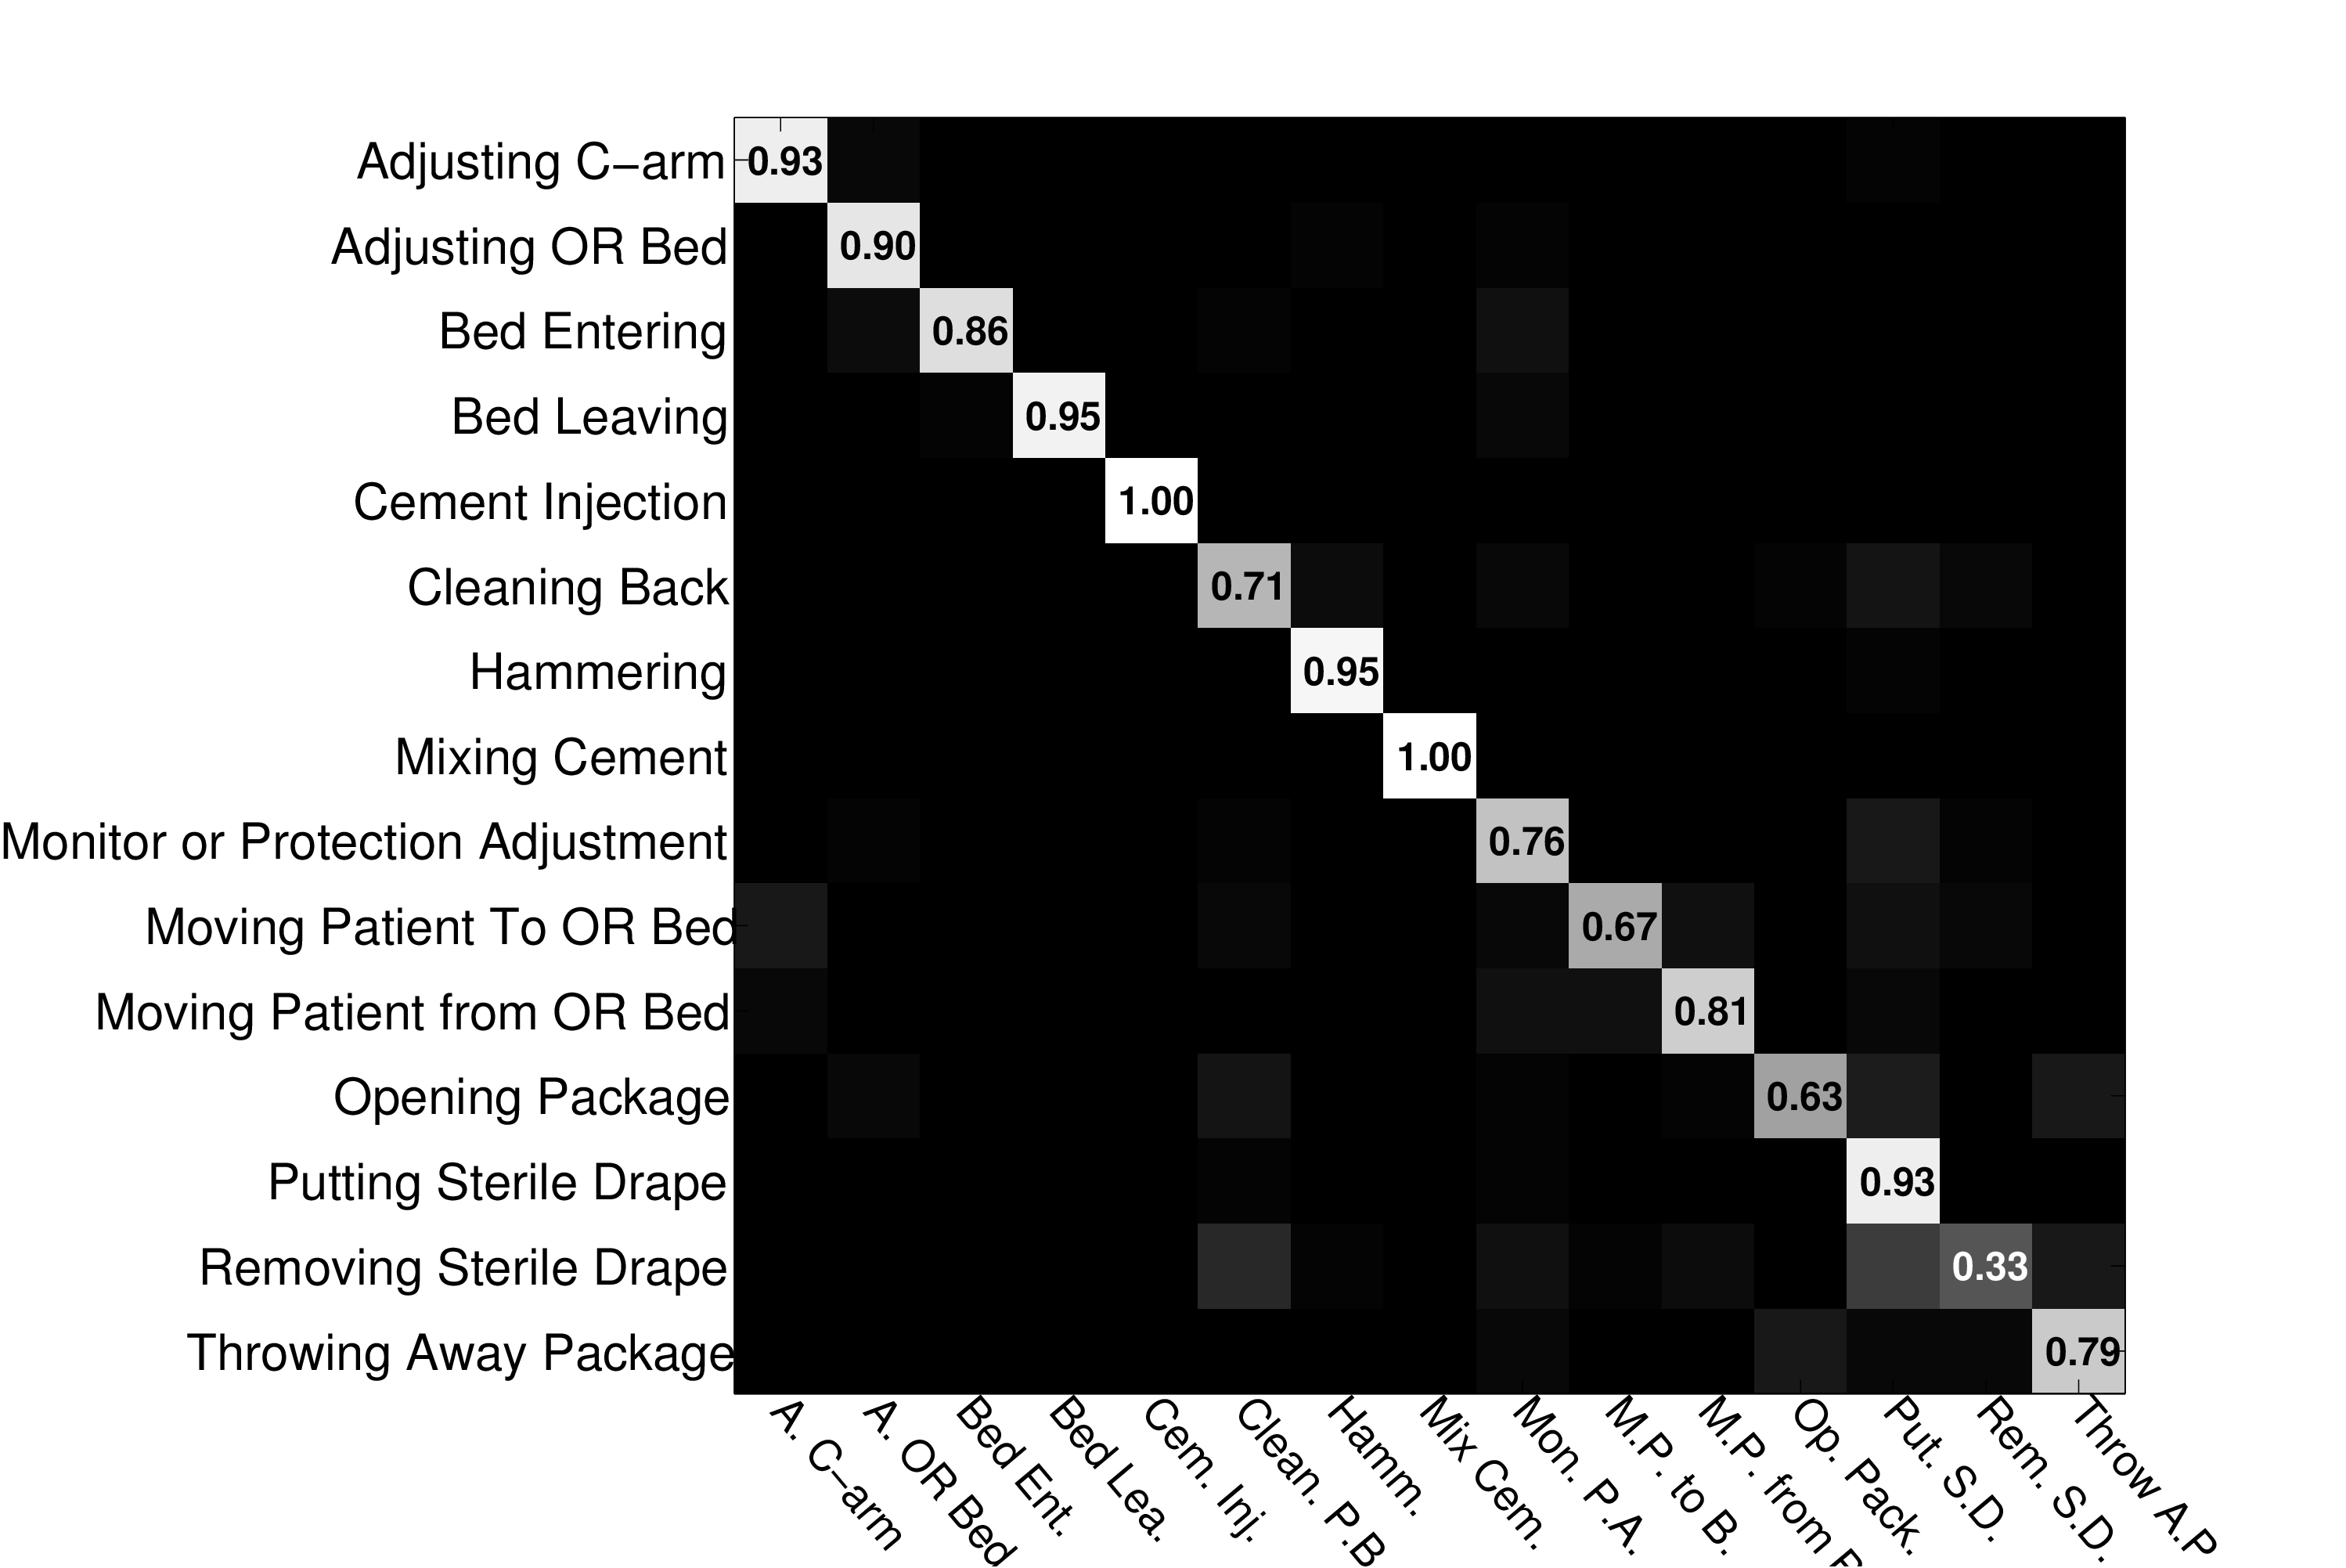
\includegraphics[scale=0.15]{Figures/confusionAndruPaper1}
\end{center}
\caption{Confusion matrix of non-voting scheme using combination of features\cite{twinanda2015data} 
\label{fig:combinationNonVotingConfusionMatrix}}
\end{figure}

In comparison of confusion matrices with voting and non-voting scheme from  Figure~\ref{fig:combinationOneModelConfusionMatrix} and Figure~\ref{fig:combinationNonVotingConfusionMatrix}, it is shown that the voting scheme has better detection on activities, i.e., Adjusting C-Arm, Adjusting OR Bed and Cleaning Back, where in these activities, detected interest points are more separable and informative than other activities. For example, in  Mixing Cement activity, 32\% accuracy decreased in voting scheme approach. In this activity, interest points are detected in very narrow space, and they detected as cluster around the activity, Thus, detected interest points are not uniform in 4D space but distributed around one point. The decrease in the accuracy can be explained as the detected interest points in 4D space is not separated informatively with non-rigid layout for the Mixing Cement activity.



















 
% Chapter 5

\chapter{Conclusions} % Main chapter title
\label{Chapter5} % For referencing the chapter elsewhere, use \ref{Chapter3} 

\lhead{Chapter 5. \emph{Conclusions}} % This is for the header on each page - perhaps a shortened title
%-----------------------------------------------------------------------------
%\section{Conclusions}
\label{section:Conclusions}
	In this thesis, a voting scheme approach is proposed to address the problem of activity recognition in an operating room using a multi-view RGBD camera system. The 4D spatio-temporal space is divided into smaller local patches using a data-driven non-rigid layout by \cite{twinanda2015data} which also helps with sparse interest points. A two-level classification strategy is introduced, i.e., learning the probability votes and learning the weights. Furthermore, two different classification approaches are compared using two-level classification: one-model and multi-model. The one-model approach trained a single classifier model with all patches from the all video clips in each level, however, the multi-model approach trained separate classifier models for  each patch type in a video clip in the fist level. Finally, the proposed voting strategy collects votes from the each local patch from a video clip and the weights are used to recognize the activity. The voting scheme is evaluated on a new dataset from \cite{twinanda2015data} which consists of annotated 1734 real surgical video clips with 15 different surgical activity types. In order to make comprehensive comparison, we compared the proposed voting scheme with non-voting scheme approach from \cite{twinanda2015data}. We have shown that the proposed voting scheme gives promising results. 
    
    The current spatio-temporal interest point detection is based on movements occur in the video clips where the detection is in the borders of the action. Hence, the detected interest points are sparse and ignore the information from stationary parts of the videos. Additionally, the bag-of-words approach is another limit which encodes the features into sparse representation. It would be interesting to incorporate extraction of dense features and different feature encoding approaches. Since the voting scheme uses local parts of 4D spatio-temporal space, it would be interesting to use the voting scheme to recognize concurrent activities.
    
    
%     The sparsity of the features because of the bag-of-words approach is addressed by introducing two level classification: first the weights of the local patches are learnt and then the learnt weights are used for training. Furthermore, two different classification approaches are compared using two-level classification: one-model and multi-model. The one-model approach trained a single model with the all patches from the all video clips, however, the multi-model approach trained separate models for the each patch type in a video clip. Finally, the proposed voting strategy collects votes from the each local patch from a video clip and a majority vote is used to recognize the activity. The voting scheme is evaluated on a new dataset from \cite{twinanda2015data} which consists of annotated 1734 real surgical video clips with 15 different surgical activity types. In order to make comprehensive comparison, we compared the proposed voting scheme with non-voting scheme approach from \cite{twinanda2015data}. We have shown that the proposed voting scheme gives promising results and is open for developing new strategies, e.g., concurrent activity recognition. The current spatio-temporal interest point detection is based on movements occur in the video clips where the detection is in the borders of the action. Hence, the detected interest points are sparse and ignoring the information from stationary parts of the videos. Additionally, the bag-of-words approach is another limit which encodes the features into sparse representation. It would be interesting to incorporate extraction of dense features and different feature encoding approaches. 
%\input{Chapters/Chapter6} 
%\input{Chapters/Chapter7} 

% Introduction

% Problem definition
% State of the art

% Methodology
% Results
% Conclusions
% Bibliography



%----------------------------------------------------------------------------------------
%	THESIS CONTENT - APPENDICES
%----------------------------------------------------------------------------------------

\addtocontents{toc}{\vspace{2em}} % Add a gap in the Contents, for aesthetics

\appendix % Cue to tell LaTeX that the following 'chapters' are Appendices

% Include the appendices of the thesis as separate files from the Appendices folder
% Uncomment the lines as you write the Appendices

% Appendix A

\chapter{The operating room} % Main appendix title

\label{AppendixA} % For referencing this appendix elsewhere, use \ref{AppendixA}

\lhead{Appendix A. \emph{Appendix Operating Room}} % This is for the header on each page - perhaps a shortened title

% \begin{center}
% 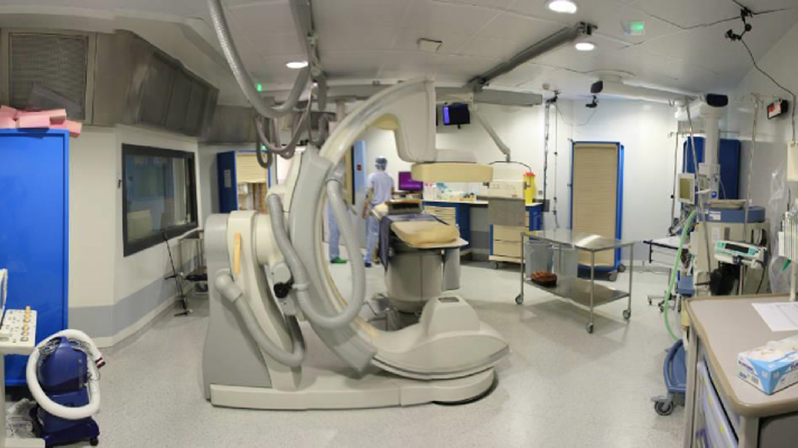
\includegraphics[scale=0.8]{Figures/CArmRoomPanaromic}
% \end{center}

\begin{figure}[here]
\centering
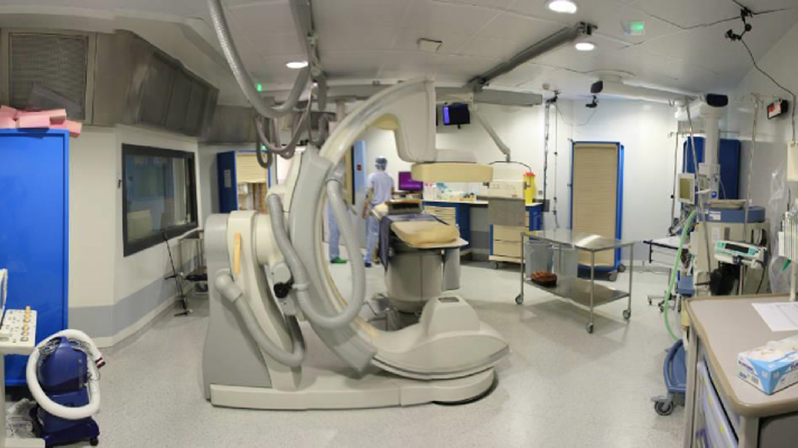
\includegraphics[width=1.0\textwidth]{Figures/CArmRoomPanaromic}
\caption{The operating room - panoramic view}
\label{fig:theOperatingRoom}
\end{figure}
%\input{Appendices/AppendixB}
%\input{Appendices/AppendixC}

\addtocontents{toc}{\vspace{2em}} % Add a gap in the Contents, for aesthetics

\backmatter

%----------------------------------------------------------------------------------------
%	BIBLIOGRAPHY
%----------------------------------------------------------------------------------------

\label{Bibliography}

\lhead{\emph{Bibliography}} % Change the page header to say "Bibliography"

\bibliographystyle{unsrtnat} % Use the "unsrtnat" BibTeX style for formatting the Bibliography

\bibliography{Bibliography} % The references (bibliography) information are stored in the file named "Bibliography.bib"

\end{document}